\documentclass{article}

% ======================
% PACKAGES
% ======================
\usepackage[a4paper,margin=1.8cm]{geometry}
\usepackage{amsmath,amssymb}
\usepackage{graphicx}
\usepackage{float}
\usepackage{caption}
\usepackage{subcaption}
\usepackage{siunitx}
\usepackage{bm}
\usepackage{mathptmx}
\usepackage{ragged2e}  % put this in the preamble
\usepackage{titlesec}
\usepackage{authblk}
\usepackage{braket}
\usepackage{multicol}
\usepackage{hyperref}
\hypersetup{
    colorlinks=true,
    linkcolor=blue,
    citecolor=blue,
    urlcolor=blue
}
%=======OUR PACKAGES================
\setlength{\columnsep}{0.6cm}
\renewcommand\thesubsubsection{\Alph{subsubsection}}
\usepackage{titlesec}

\titleformat{\section}
  {\centering\normalfont\Large\bfseries}
  {\thesection}{0.5em}{}

\titleformat{\subsection}
  {\centering\normalfont\large\bfseries}
  {\thesubsection}{0.5em}{}

\titleformat{\subsubsection}
  {\centering\normalfont\normalsize\bfseries}
  {\thesubsubsection}{0.5em}{}

%====================================

% ======================
% TITLE
% ======================
\title{\textbf{Monte Carlo Simulation of the 2D Ising Model}}
\author{Konstantinos Pourgourides$^{\dagger}$, Kyproula Mitsidi$^{\dagger}$}
\affil{\small $\dagger$ Faculty of Applied Sciences, Delft University of Technology, Lorentzweg 1, 2628 CK, Delft, The Netherlands}
\date{}

% ======================
% DOCUMENT
% ======================
\begin{document}

\maketitle
\vspace{-2.5em}
\begin{center}
\textbf{ABSTRACT}\\
\vspace{0.7\baselineskip}
\begin{minipage}{0.8\textwidth}

We present a Monte Carlo simulation of the 2D Ising Model
on a square spin lattice using the Metropolis Algorithm. We discuss the underlying physical and mathematical principles of the simulation and perform validation tests to ensure its reliability. Physical observables including magnetization, energy, susceptibility, and specific heat are investigated as functions of temperature, with particular emphasis on their behavior near the critical temperature, where nontrivial phenomena emerge. We additionally study the effect of an external magnetic field on the magnetization. The numerical results are found to be consistent with the analytical solution of the model, supporting the validity of the implemented methods. Moreover, we quantify how the computational time scales with the dimension of the spin lattice and the Monte Carlo cycles, providing insights on the simulation performance. Finally, we conduct a detailed efficiency comparison between the standard and the numpified Metropolis Algorithm, demonstrating how the performance gains from the latter can help us reveal more accurate physics by approaching the thermodynamic limit more efficiently.

\end{minipage}
\end{center}
\vspace{0.5\baselineskip}
% ======================
\begin{multicols}{2}
% ======================

\section{Introduction}

The Ising Model serves as a simple but insightful description of (anti-)ferromagnetism, as it models interactions between neighboring spins under the influence of an external magnetic field. Spins can be either in the ``up" or ``down" state, and interactions occur only between the nearest neighbors. The system tends to favor lower energy configurations by aligning the spins; on the other hand, heat is able to produce disturbances that result in different structural phases, in some cases exhibiting a phase transition between an ordered and disordered state.\\

The model was first introduced around 1920 by Wilhelm Lenz as a problem to his student Ernst Ising, who solved the 1D model for his doctoral thesis in 1924. The 2D model was solved by Lars Onsager (for no external magnetic field) in 1944, exhibiting a phase transition at a certain critical temperature \cite{onsager}. Despite significant progress in statistical mechanics, no analytical solution is known for the 2D model in a non-zero magnetic field, or higher dimensions regardless of the presence of the field.\\

Despite the mathematical elegance and simplicity of the model, it is able to capture the collective behavior, interactions and phase transitions of multiple entities in complex dynamical systems. For this reason, it is widely used in a variety of physics areas, such as statistical mechanics, condensed matter physics, and high-energy lattice theories.

\vspace{-1em}
% ======================
\section{Theory}

In this section, we present the underlying theory regarding the Ising Model and algorithmic techniques utilized to simulate it, which will serve as a steppingstone for the next sections \cite{computational_book}.

\subsection{The 2D Ising Model}
\label{sec_ising}

The 2D Ising Model consists of a square spin lattice configuration $\bm{\Lambda}$ with $N =L\times L$ sites ($N \to \infty$ in the thermodynamic limit), where spins can assume values $\pm 1$ corresponding to the ``up" and ``down" states. A spin labeled by index $\mathbf{x}=(i,j)$, $s_{\mathbf{x}}$, is located on lattice site $\boldsymbol{\Lambda}_{i,j}, \ \forall i,j \in\{0,\dots,L-1\}$, and $\langle \mathbf{xy} \rangle$ denotes a nearest neighbor pair of spins $s_{\mathbf{x}},s_{\mathbf{y}}$. The nearest neighbors of a spin $s_{\mathbf{x}}$ are located directly above ($\boldsymbol{\Lambda}_{i-1,j}$), below ($\boldsymbol{\Lambda}_{i+1,j}$), left ($\boldsymbol{\Lambda}_{i,j-1}$) and right ($\boldsymbol{\Lambda}_{i,j+1}$) with respect to lattice site $\boldsymbol{\Lambda}_{i,j}$. In the presence of an external magnetic field $H$, the Hamiltonian for a certain configuration of the system is

\begin{equation}
    \mathcal{H}(\boldsymbol{\Lambda}) = -J\sum_{\langle \mathbf{xy}\rangle} s_{\mathbf{x}}s_\mathbf{y} - H\sum_{\mathbf{x}}{s_{\mathbf{x}}},
    \label{hamiltonian}
\end{equation}
%
where J is the coupling strength between nearest neighbor spins. The system prefers configurations that lower the total energy, and thus for $J>0$ ($J<0$), the coupling term favors aligned (anti-aligned) spins, a phenomenon known as ferromagnetism (anti-ferromagnetism); the magnetic term favors spins with the same sign as the external magnetic field. The partition function $Z$ of the system is given by

\begin{align}
    Z = \sum_{\boldsymbol{\Lambda}}e^{-\beta\mathcal{H}(\boldsymbol{\Lambda})} = 
    \sum_{\boldsymbol{\Lambda}}\exp\left[ \beta J\sum_{\langle \mathbf{xy} \rangle} s_{\mathbf{x}}s_{\mathbf{j}} + \beta H\sum_{\mathbf{x}}{s_\mathbf{x}}  \right],
\end{align}
%
where $\beta = 1/k_BT$. We restrict our discussion to the case of no external magnetic field ($H=0$), for which the model admits an analytical solution.\\

We turn our attention to magnetization, defined as

\begin{align}
    m(\boldsymbol{\Lambda}) = \frac{1}{N}\sum_{\mathbf{x}}
s_{\mathbf{x}} \end{align}
%
and study its behavior for different temperatures. Near absolute zero $\beta \to \infty$ $(T \to 0)$, all spins are either ``up" or ``down" after a sufficiently long time, and $m(\boldsymbol{\Lambda}) = \pm1$. Considering the configuration in which all the spins are in the ``up" state, the flip probability for a spin $s_{\mathbf{x}}$ (see section \ref{section_metropolis}) is 

\begin{align}
    P_{\mathbf{x}}^{\text{flip}}(\beta) 
    = \exp\left[-\beta Js_{\mathbf{x}}\left(2\sum_{\langle \mathbf{xy} \rangle}s_{\mathbf{y}}\right)\right]
    = \exp(-8\beta J) \approx 0,
\end{align}
%
making a spin flip event very rare at low temperatures. In the opposite regime of high temperatures $\beta \to 0$ $(T \to \infty)$, all spin flips are accepted, and therefore all configurations are equiprobable, with spins assuming values $\pm 1$ randomly. In that case, $m(\boldsymbol{\Lambda}) \approx 0$.\\

The Hamiltonian $\mathcal{H}(\boldsymbol{\Lambda})$ is invariant under a global spin flip at any temperature. However, the magnetization is not invariant under the same transformation as $m(-\boldsymbol{\Lambda}) = -m(\boldsymbol{\Lambda})$. Evidently the system exhibits symmetry breaking, as there is a non-zero magnetization in the equilibrium state for $T\to 0$, whereas for $T\to\infty$, the symmetry is restored, as $m(\boldsymbol{\Lambda}) \to 0$.\\

The preceding discussion implies that the magnetization either decays to zero asymptotically, or drops to zero at a certain critical temperature $T_c$. Indeed, in the thermodynamic limit $N \to \infty$ the magnetization vanishes abruptly, but continuously, at a critical temperature given by

\begin{align}
    \frac{k_BT_c}{J} = \frac{1}{\ln{(1+\sqrt{2})}} \approx 2.269.
\end{align}
%
This is a characteristic behavior of a second order phase transition, and the order parameter is magnetization. Such transitions are characterized by a smooth free energy $\mathcal{F} = -k_BT\ln{Z}$ at the transition point with continuous first derivatives, such as the magnetization

\begin{align}
    m(T) = -\frac{\partial \mathcal{F}}{\partial H}\Bigg|_{H=0}.
\end{align}
%
On the other hand, second derivatives such as the specific heat $C$ and magnetic susceptibility $\chi$, diverge at the transition point

\begin{align}
    C(T) = -\frac{T}{N}\frac{\partial^2\mathcal{F}}{\partial T^2}\Bigg|_{H=0},
    \quad
    \chi(T) = -\frac{\partial^2\mathcal{F}}{\partial H^2}\Bigg|_{H=0}.
\end{align}
%
More specifically, near the transition point, these quantities behave as following \cite{computational_book}

\begin{align}
    &C(T) \propto -\ln|T-T_c|^{-\alpha} \label{c}, \\
    \nonumber \\
    &m(T) \propto (T_c-T)^{\beta}, \quad T/T_c < 1 \label{m},\\
    \nonumber \\
    &\chi(T) \propto |T-T_c|^{-\gamma} \label{x},
\end{align}
%
where $\alpha=0$, $\beta=1/8$ and $\gamma=7/4$ are the critical exponents. The singular behavior of these thermodynamic quantities is closely related to the emergence of long-range correlations in the system. As $T\to T_c$, spins become correlated over increasingly large distances, leading to the formation of spin domains of varying sizes, resulting in large fluctuations in magnetization and energy.\\

When simulating the Ising Model, we calculate observables as weighted averages over different spin configurations $\boldsymbol{\Lambda}$, where the probability $P(\boldsymbol{\Lambda})$ of each configuration is given by the normalized Boltzmann factor

\begin{align}
    \langle A\rangle = \sum_{\boldsymbol{\Lambda}}P(\boldsymbol{\Lambda}) A(\boldsymbol{\Lambda}) = 
    \frac{1}{Z}\sum_{\boldsymbol{\Lambda}}A(\boldsymbol{\Lambda})e^{-\beta \mathcal{H}(\boldsymbol{\Lambda})}.
    \label{A}
\end{align}
%
For $N$ spins, we would have to sum over all $2^N$ possible configurations to calculate $\langle A\rangle$, which is practically impossible as $N \to \infty$. Obviously, configurations are not equiprobable, as those with lower energies are exponentially more likely to occur. For the majority of the time, the system is in one of few (compared to $2^N$) highly probable configurations, while occasionally visiting less likely, high energy configurations. Due to this, we can approximate the sum of Eq. \eqref{A} as a sum over typically visited configurations with the help of Monte Carlo Markov Chains.

\subsection{Markov Chain Monte Carlo}

In Markov Chains \cite{montecarlo}, we have a sequence of spin configurations $\{\boldsymbol{\Lambda}\} = \boldsymbol{\Lambda}^1,\dots,\boldsymbol{\Lambda}^k$ corresponding to subsequent iterations. The probability of transitioning from a randomly chosen configuration $\boldsymbol{\Lambda}^i$ to $\boldsymbol{\Lambda}^{i+1}$ depends only on $\boldsymbol{\Lambda}^i$. The transition probability between different configurations is denoted as $T(\boldsymbol{\Lambda}\to \boldsymbol{\Lambda}')$, and normalization demands that $\sum_{\boldsymbol{\Lambda}'}T(\boldsymbol{\Lambda}\to \boldsymbol{\Lambda}') = 1$. The probability of a configuration $\boldsymbol{\Lambda}$ occurring in iteration $i+1$ is given by

\begin{align}
    P_{i+1}(\boldsymbol{\Lambda}) &= \nonumber \\ 
    &+ P_i(\boldsymbol{\Lambda}) \quad \text{probability of already being in } \boldsymbol{\Lambda}, \nonumber \\
    &- \sum_{\boldsymbol{\Lambda}'}P_i(\boldsymbol{\Lambda})T(\boldsymbol{\Lambda} \to \boldsymbol{\Lambda}')  \quad \text{probability of flowing out of } \boldsymbol{\Lambda}, \nonumber \\
    &+ \sum_{\boldsymbol{\Lambda}'}P_i(\boldsymbol{\Lambda}')T(\boldsymbol{\Lambda}'\to \boldsymbol{\Lambda})  \quad \text{probability of flowing into } \boldsymbol{\Lambda}.
    \label{mastereq}
\end{align}
%
We want to sample from the same probability distribution in all iterations, i.e. $P_{i+1}(\boldsymbol{\Lambda}) = P_i(\boldsymbol{\Lambda})$, which simplifies Eq. \eqref{mastereq} to 

\begin{align}
    \sum_{\boldsymbol{\Lambda}'}P(\boldsymbol{\Lambda})T(\boldsymbol{\Lambda} \to \boldsymbol{\Lambda}') =
    \sum_{\boldsymbol{\Lambda}'}P(\boldsymbol{\Lambda}')T(\boldsymbol{\Lambda}'\to \boldsymbol{\Lambda}).
\end{align}
%
A particular solution known as \textbf{detailed balance} is given by

\begin{align}
    P(\boldsymbol{\Lambda})T(\boldsymbol{\Lambda} \to \boldsymbol{\Lambda}') =
    P(\boldsymbol{\Lambda}')T(\boldsymbol{\Lambda}'\to \boldsymbol{\Lambda}).
    \label{mastereq2}
\end{align}
%
It all boils down to choosing the appropriate transition probabilities in order to generate the desired probability distribution $P(\boldsymbol{\Lambda})$. The Metropolis algorithm will help us solve this issue.

\subsection{Metropolis Algorithm}
\label{section_metropolis}

In the Metropolis algorithm \cite{computational_book}, we consider the transition probability $T(\boldsymbol{\Lambda}\to \boldsymbol{\Lambda}') = \omega_{\boldsymbol{\Lambda}\boldsymbol{\Lambda}'}A_{\boldsymbol{\Lambda}\boldsymbol{\Lambda}'}$. Starting from configuration $\boldsymbol{\Lambda}$, we create a candidate configuration $\boldsymbol{\Lambda}'$ with probability $\omega_{\boldsymbol{\Lambda}\boldsymbol{\Lambda}'}$. This trial move is accepted with probability $A_{\boldsymbol{\Lambda}\boldsymbol{\Lambda}'}$. The situation is further simplified if we consider symmetric probabilities for the trial move (i.e. $\omega_{\boldsymbol{\Lambda}\boldsymbol{\Lambda}'}=\omega_{\boldsymbol{\Lambda}'\boldsymbol{\Lambda}}$), such that Eq. \eqref{mastereq2} becomes $P(\boldsymbol{\Lambda})A_{\boldsymbol{\Lambda}\boldsymbol{\Lambda}'}=P(\boldsymbol{\Lambda}')A_{\boldsymbol{\Lambda}'\boldsymbol{\Lambda}}$. The solution given in \cite{metropolis} is

\begin{align}
    A_{\boldsymbol{\Lambda}\boldsymbol{\Lambda}'} = 
    \begin{cases}
        1, &P(\boldsymbol{\Lambda}')>P(\boldsymbol{\Lambda})\\
        \frac{P(\boldsymbol{\Lambda}')}{P(\boldsymbol{\Lambda})}, &P(\boldsymbol{\Lambda}')<P(\boldsymbol{\Lambda}).
    \end{cases}
\end{align}
%
In the context of the Ising Model, the proposed trial move is the flip of a spin, and the probability of accepting this move is given by

\begin{align}
    A_{\boldsymbol{\Lambda}\boldsymbol{\Lambda}'} = 
    \begin{cases}
        1, &E(\boldsymbol{\Lambda}')<E(\boldsymbol{\Lambda})\\
        \exp(-\beta\Delta E), &E(\boldsymbol{\Lambda}')>E(\boldsymbol{\Lambda}),
    \end{cases}
    \label{rule}
\end{align}
%
where $E(\boldsymbol{\Lambda)}$ is the energy of configuration $\boldsymbol{\Lambda}$, and $\Delta E$ is the energy difference between the proposed and current spin configurations. In summary, the Metropolis algorithm for simulating the Ising model is composed of the following steps:

\begin{itemize}
    \item[I] Start with a spin configuration $\boldsymbol{\Lambda}$;
    \item[II] Take $\boldsymbol{\Lambda}$ and flip a randomly chosen spin to create a candidate configuration $\boldsymbol{\Lambda}'$;
    \item[III] If $\boldsymbol{\Lambda}'$ lowers the energy of the system with respect to $\boldsymbol{\Lambda}$ accept the move, otherwise accept it with probability $\exp(-\beta\Delta E)$;
    \item[IV] Repeat starting from the most recently accepted configuration until a certain number of iterations is reached.
\end{itemize}

\section{Methods}

\subsection{Simulation Setup}

The basis of the simulation is the square spin lattice $\boldsymbol{\Lambda}$, otherwise the spin grid. It consists of $N=L\times L$ sites, each one equipped with a spin. The model parameters that influence the behavior of the spin grid during the simulation are its dimension $L$, the temperature $T$, the nearest-neighbor coupling strength $J$, and the external magnetic field $H$. 

\subsection{Initialization}

The initialization of the simulation is based on the initial configuration of the spin grid. The spins can either be chosen randomly at each site, or fully aligned. Alternatively, the simulation provides the possibility of a custom spin grid input. Intuitively, starting from an aligned spin grid will benefit the tendency of the system to be in an ordered state; nevertheless, heat can still cause local structural fluctuations (i.e., spin flips).

\subsection{Time Evolution}

Starting from the initial configuration, the system will evolve according to the Hamiltonian in Eq. \eqref{hamiltonian}. The time evolution takes place over a certain number of intervals, referred to as Monte Carlo (MC) cycles, denoted by $n$. Every MC cycle consists of N iterations; in each iteration, a spin is randomly chosen and proposed to flip. The proposal will be accepted or not based on the rule we defined in Eq. \eqref{rule}, with the deciding factor being the energy shift $\Delta E$ between the proposed and current configuration. 

\subsubsection{Neighboring Interactions \& Boundary Conditions}

The energy shift depends on the interactions between a spin and its nearest neighbors, located directly above, below, to the left and to the right of the spin site. The system is subject to periodic boundary conditions, and as a result, the first and last spin of every row ($\boldsymbol{\Lambda}_{i,0} \leftrightarrow\boldsymbol{\Lambda}_{i,L}$) and column ($\boldsymbol{\Lambda}_{0,j} \leftrightarrow\boldsymbol{\Lambda}_{L,j}$) of the spin grid are considered as neighbors. A proposed spin configuration in which a randomly chosen spin flips, amounts to an energy shift $\Delta E$ given by

\begin{align}
    \Delta E = 2s_\mathbf{x}(J\sum_{\braket{\mathbf{xy}}}s_\mathbf{y} + H).
    \label{shift}
\end{align}

\subsubsection{Metropolis criterion}

If the proposed spin configuration lowers the total energy of the system it is instantly accepted ($P=1$), otherwise it is accepted with probability $P = e^{-\beta \Delta E}$.

\subsubsection{Equilibration}

The simulation of the Ising Model eventually aims at the study of observables, which are calculated by taking averages over different spin configurations. The system is initialized in an artificial configuration, which is iteratively shaped towards reality by the interactions, temperature, and external magnetic field of the system. For this reason, we omit a certain number of initial MC cycles in our calculations, denoted as $n_0$\footnote{This implies that observables are averaged over $n-n_0$ MC cycles.}, to let the system evolve towards thermal equilibrium. This is achieved by allowing fluctuations to develop correctly, spins to rearrange, and domains to form or dissolve. The specific criterion of equilibration will be discussed in section 4.1.\ref{sec_equilibrium} in further detail. 

\subsection{Observables}

As established in section \ref{sec_ising}, observables are calculated as averages over the visited spin configurations during the time evolution, which corresponds to an average over MC cycles

\begin{align}
    \braket{A} = \frac{1}{n-n_0}\sum_{i>n_0}^{n}A_i,
    \label{observables}
\end{align}
%
where $A_i$ is the value of the observable following the i-th MC cycle. Apart from the energy per spin (Eq. \eqref{hamiltonian}), the observables calculated in the simulation are the magnetization, the specific heat per spin, and the susceptibility per spin. The following discussion on the observables assumes no external magnetic field, for which the model admits an analytical solution. We will focus on the behavior of the observables in the regimes of low temperatures $T/T_c<<1$, large temperatures $T/T_c>>1$ and at the critical temperature $T/T_c=1$, where interesting effects emerge due to the formation of clusters across the spin grid, resulting in irregular fluctuations and divergencies (Fig. (\ref{cluster})). An investigation for the case of non-zero magnetic field will take place in section \ref{sec_magnetic}.

\begin{figure}[H]
    \centering
    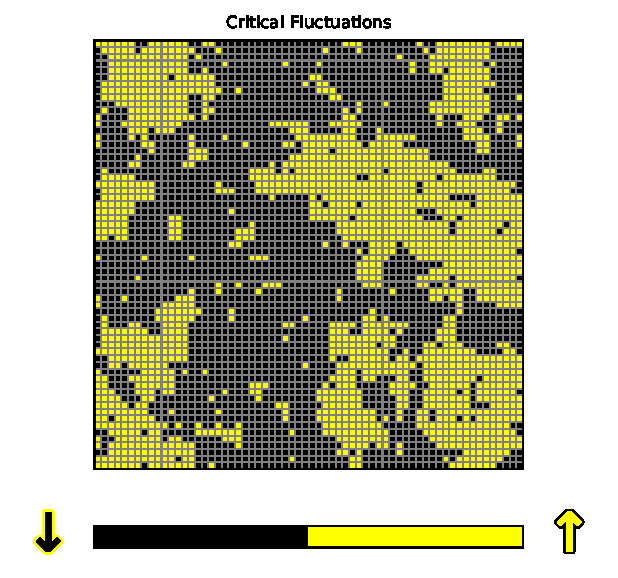
\includegraphics[width=\columnwidth]{plots/spingrid_clusters.pdf}
    \caption{A snapshot of the spin grid configuration for $\{L,J,H,n-n_0\}=\{64, 1,0,15000\}$ at the critical temperature. In this regime, large spin domains form across the lattice, demonstrating the critical fluctuations associated with the phase transition and the instability of the system.}
    \label{cluster}
\end{figure}

\subsubsection{Magnetization}

The absolute magnetization is given by

\begin{align}
    \braket{m} = \frac{1}{N} \braket{\sum_\mathbf{x}s_\mathbf{x}} \in [0,1].
\end{align}
%
In the limit of low temperatures $T/T_c<<1$, spins are mostly aligned, making flips highly improbable but not impossible, resulting in small fluctuations. This state is known as ferromagnetic ($J>0$) or anti-ferromagnetic ($J<0$), with $\braket{m} \to \pm1$ or $\braket{m} \to 0$ respectively. In the limit of high temperatures $T/T_c>>1$, spin flips are always accepted, driving the system towards a random state, where $\braket{m}\to 0$. At $T/T_c=1$, the absolute magnetization vanishes continuously as in Eq. \eqref{m}.

\subsubsection{Specific Heat per spin}

The specific heat per spin is given by

\begin{align}
    \braket{C} =
\frac{k_B \beta^2}{N} \left( \langle E^2 \rangle - \langle E \rangle^2
\right).
\end{align}
%
This quantity is a measure of the energy fluctuations. In the limit of low temperatures $T/T_c<<1$, mostly aligned spins and small flip probabilities keep the energy fluctuations under control, resulting in a smooth and small specific heat. In the limit of high temperatures $T/T_c>>1$, thermal energy dominates over interaction energy, and spins are aligned randomly; the total energy of the system fluctuates slightly around a constant value, and the specific heat is again small. At $T/T_c=1$, large energy fluctuations cause a logarithmic divergence to the specific heat, as in Eq. \eqref{c}.

\subsubsection{Susceptibility per spin}

The susceptibility per spin is given by

\begin{align}
    \braket{\chi} = \beta N \left(
\langle m^2 \rangle - \langle m \rangle^2 \right).
\end{align}
%
This quantity is a measure of magnetization fluctuations. In the limit of low temperatures $T/T_c<<1$, $\braket{m} \to \pm1$ with small fluctuations due to almost fully aligned spins, resulting in a small susceptibility. In the limit of high temperatures $T/T_c>>1$, $\braket{m} \to 0$ with small fluctuations because spins are randomly aligned, resulting again in small susceptibility. At $T/T_c=1$, huge magnetization fluctuations cause the susceptibility to diverge as a power law, as in Eq. \eqref{x}.

\subsection{Errors}

For the simulation data, we estimate the errors using a combination of the Autocorrelation and Bootstrap methods. The next subsection is dedicated to a more detailed analysis of the aforementioned techniques.

\subsubsection{Autocorrelation}
The error of the quantity in Eq. \eqref{observables} cannot be estimated using the well-known formula for the standard deviation
\begin{equation}
 \sigma_A = \sqrt{\frac{1}{(n-n_0)-1}\sum^n_{i>n_0}\left(A_i - \langle A \rangle \right)^2},
\end{equation}
as the data we obtain in the simulation are correlated; the state of the system in a time step depends on the previous. To obtain a statistically uncorrelated dataset we use the autocorrelation function \cite{computational_book}, defined as

\begin{equation}
\chi_A(t) =
\frac{\langle A_i A_{i+t} \rangle - \langle A_i \rangle \langle A_{i+t} \rangle}
{\sqrt{ \left(  \langle A_i^2 \rangle - \langle A_i \rangle^2\right)\times \left( \langle A_{i+t}^2 \rangle - \langle A_{i+t} \rangle^2\right)}},
\end{equation}
with 
\begin{align}
    &\langle A_i \rangle \equiv \frac{1}{(n-n_0)-t} \sum_{i>n_0}^{(n-n_0)-t} A_i,\\
    &\langle A_{i+t} \rangle \equiv \frac{1}{(n-n_0)-t} \sum_{i>n_0}^{(n-n_0)-t} A_{i+t}.
\end{align}
%
The autocorrelation function has the form of an exponential decay $e^{-t/\tau}$, where $\tau$ is the correlation time. Essentially, it is the least number of MC cycles that must separate two measurements to become statistically independent. By fitting the decay, we can determine $\tau$ and calculate the error of our observable as

\begin{equation}
    \sigma_A = \sqrt{\frac{2 \tau}{n-n_0} \left(\langle A^2 \rangle - \langle A \rangle^2\right)} \ .
\end{equation}



\subsubsection{Bootstrap}

Observables that depend on the fluctuations of other quantities have considerably larger uncertainties, such as the specific heat and susceptibility, which depend on the fluctuations of energy and magnetization respectively. To calculate the errors of these quantities we use a combination of the Autocorrelation and Bootstrap \cite{Bootstrap} methods.\\

Initially, we calculate the correlation time for the fluctuating observable (e.g. energy), and then approximate a de-correlated dataset by retaining measurements separated by $\tau$ MC cycles, resulting in $n_d$ data points. Then, we randomly draw $n_d$ data points from the de-correlated dataset to generate a new sample $k^i$. We repeat this process for $n_b$ times ($n_b>>1$) in total. For each sample in $k = \{k^1,\dots,k^{n_b}\}$, we compute the variance of the observable, and then multiply with the appropriate constants to obtain the desired quantity $A_k = \{A^1,\dots,A^{n_b} \}$ (e.g. specific heat in Eq. \eqref{c}). The error of $A$ is estimated through

\begin{equation}
    \sigma_A = \sqrt{\langle A^2 \rangle - \langle A \rangle^2} 
\end{equation}

\noindent where the averages are taken over the set $A_k$. 

\subsection{Numpified Version Extension}

The simulation goes beyond the initial implementation of the standard Metropolis Algorithm, and employs a more efficient variant, namely the Numpified Metropolis Algorithm.\\

The main idea behind the algorithm is the following: the energy shifts $\Delta E$ that dictate whether proposed configurations will be accepted or not, are based solely on nearest neighbor interactions. If we imagine the spin grid as a black-and-white checkerboard, the nearest neighbors of all white sites are black  sites and vice versa, without any interactions occurring between same-colored sites. The situation is illustrated in Fig. (\ref{chessboard}) using an AI-generated picture for further clarity.\\

This allows for the trial move being simultaneously proposed and tested for all black, and then all white sites, or vice versa. Keeping this in mind, we can reduce the number of iterations from $N$ to 2 per MC cycle. In a spin grid $\boldsymbol{\Lambda}$, black and white sites are computationally distinguished through their row and column indices

\begin{align}
    (i+j)\mod 2 = 0 \rightarrow \text{black site,} \nonumber \\
    \label{latticeselect} \\
    (i+j)\mod 2 = 1 \rightarrow \text{white site}. \nonumber
\end{align}
%
The energy shift can now be represented by an $L\times L$ matrix $\boldsymbol{\Delta \tilde{E}}$, where each element $\boldsymbol{\Delta \tilde{E}}_{i,j}$ corresponds to the respective energy shift, given by Eq. \eqref{shift}, that would occur by the flipping the spin at lattice site $\boldsymbol{\Lambda}_{i,j}$ \\

The Metropolis criterion can also be vectorized in a similar fashion, by constructing an $L\times L$ Boltzmann matrix $\boldsymbol{\tilde{B}} \equiv \exp(-\beta \boldsymbol{\Delta \tilde{E}})$ and comparing it to an $L\times L$ random matrix $\boldsymbol{\tilde{R}}$, with values distributed uniformly in $[0,1]$. Therefore, a proposed flip at spin site $\boldsymbol{\Lambda}_{i,j}$ is accepted if the following conditions hold

\begin{align}
\boldsymbol{\Delta \tilde{E}}_{i,j} < 0 \quad &\textbf{or}\quad \ \boldsymbol{\tilde{R}}_{i,j} < \boldsymbol{\tilde{B}}_{i,j}.
\end{align}
%
By utilizing matrix multiplications through NumPy (and hence the name ``numpified"), we can check the Metropolis criterion for all white and black sites simultaneously, by filtering lattice sites using the conditions of Eq. \eqref{latticeselect}. The improved efficiency of this algorithm will allow for the exploration of larger spin grids for more MC cycles, in comparison to the standard algorithm. Further comments on the efficiency of the numpified and standard Metropolis Algorithms are discussed in section \ref{sec_performance}. 

\begin{figure}[H]
    \centering
    
\includegraphics[width=\columnwidth]{plots/chess_board.png}
    \caption{The spin grid re-imagined as a black-and-white checkerboard, where neighboring interactions occur only between opposite-colored sites, allowing for the simultaneous proposal of the trial move to all same-colored sites. This image was generated with chatGPT.}
    \label{chessboard}
\end{figure}

\section{Results}

\subsection{Validation Checks}

We perform some validation checks on the initialization of the spin grid $\boldsymbol{\Lambda}$, as well as the equilibration time $n_0$, to ensure that the simulation works as intended. 

\subsubsection{Initialization}

The spin grid can be initialized in a random or fully aligned configuration; an example for each of these choices is illustrated in Fig. (\ref{spingrid}) for $L=64$.

\begin{figure}[H]
    \centering
    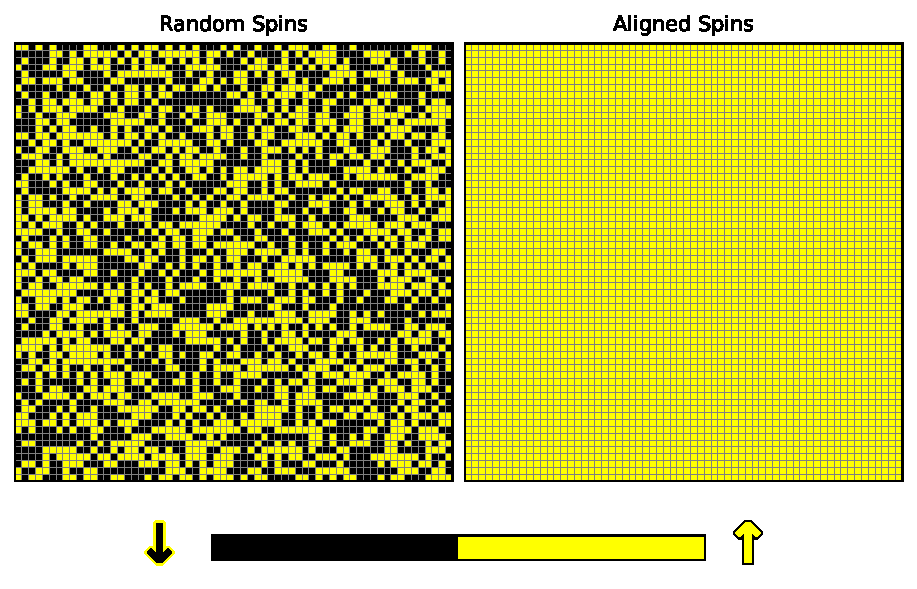
\includegraphics[width=1\columnwidth]{plots/spingrid.pdf}
    \caption{A randomized and a fully aligned initial spin grid configuration for $L=64$.}
    \label{spingrid}
\end{figure}

The results are visually convincing, but we also compute the magnetization for further confirmation, and we find that $    m(\boldsymbol{\Lambda_\text{random}}) < 1\times10^{-3}$ and  $m(\boldsymbol{\Lambda_\text{aligned}}) = 1$, which signifies the correctness of the initialization. The magnetization of the random configuration is non-zero due to the finite size of the system; in the thermodynamic limit $N\to\infty$, it will vanish completely.


\subsubsection{Time evolution}
\label{sec_equilibrium}

After the spin grid has been initialized, it takes some MC cycles until equilibration is reached. To find the equilibration time $n_0$, we study the evolution of magnetization \cite{Jaschke}, which reflects the status of the spin grid. We expect to see the system relaxing from its initial state, and start fluctuating around a stable value as it reaches equilibrium. If we average over multiple simulation runs and additionally smooth the data with a Gaussian filter, we observe the magnetization stabilizing completely upon equilibrium. \\

Initially, we explore the evolution of magnetization for different temperatures. We perform 35 independent simulation runs for 13 different temperatures using a fixed spin grid dimension. The preceding is depicted in Fig. (\ref{evol abs mag diff temp}), from which several important observations can be made. Firstly, as temperature increases, the system tends to fluctuate around lower magnetization values. We can see that for $T/T_c<1$, the domain of interest is around $|m| \approx 0.8-1.0$, indicating strong spin ordering (e.g. Fig. (\ref{spingrid}), right). For $T/T_c>1$, thermal fluctuations dominate and the domain is shifted around $|m| \approx 0.0-0.2$, corresponding to a disordered spin grid (e.g. Fig. (\ref{spingrid}), left). For $T/T_c \approx 1$, the intermediate values are preferred, reflecting the transition between the two regimes; clusters of aligned spins continuously form and dissolve (e.g. Fig. (\ref{cluster})). \\

Additionally, we can see that for $T/T_c <1$, the system reaches equilibrium after a finite amount of time, whereas for $T/T_c > 1$ the magnetization stabilizes almost immediately. For $T/T_c \approx 1$, the system exhibits fluctuations and a critical slow down. In this regime, magnetization does not settle to a single well-defined value, due to the spin cluster formation and dissolution.

\begin{figure}[H]
    \centering
    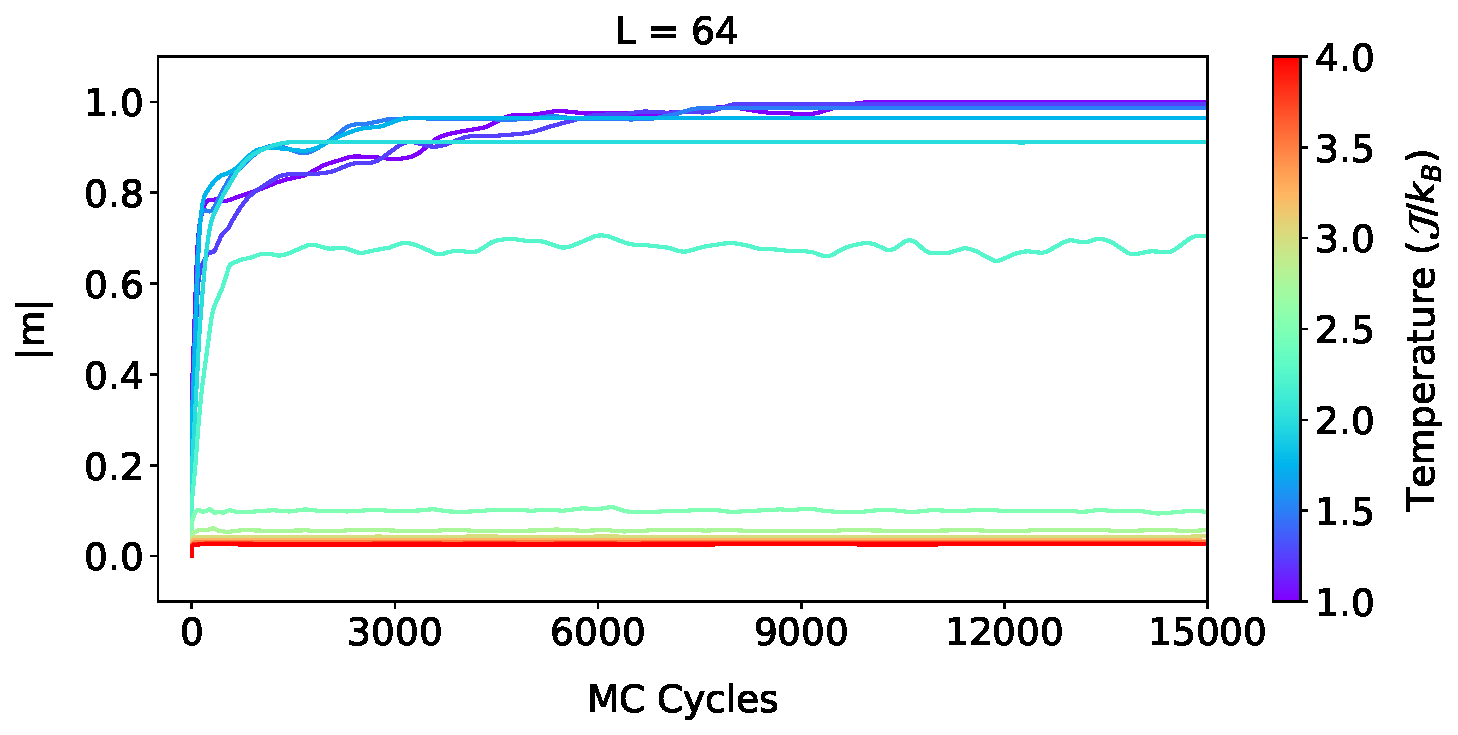
\includegraphics[width=1\columnwidth]{plots/m_vs_mc_diff_temper.pdf}
    \caption{Evolution of absolute magnetization for different temperatures in the range $[1.0,4.0] \ J/k_B$ in increments of $0.25 \ J/k_B$ and fixed spin grid dimension $L = 2^{6}$ (randomized initial conditions). The data are averaged over 35 simulations and the noise has been filtered out.}
    \label{evol abs mag diff temp}
\end{figure}


Due to the aforementioned behavior, the equilibration time $n_0$ is studied for $T/T_c < 1$. We perform 35 independent simulations for 6 different temperatures over 4 spin grid dimensions. To determine $n_0$, we identify the smallest Monte Carlo step $i$ such that the condition

\begin{equation}
\left||m_i| - |m_{i+15}|\right| < 7 \times 10^{-5}
\label{condition}
\end{equation}

\noindent is satisfied for a window of 750 consecutive cycles, and we define $n_0 = i + 750$.
%
The parameters and thresholds in this criterion have been calibrated to ensure that $n_0$ is found reliably without misinterpreting local plateaus as equilibration.\\


The absolute magnetization evolution for the different spin grids is depicted in Fig. (\ref{n0_nump}). If the results were not averaged over multiple runs and smoothed using a Gaussian filter, the magnetization trajectories would exhibit large statistical fluctuations, particularly for smaller spin-grid sizes. This is expected, as the impact of a spin flip is inversely proportional to the spin grid dimension. Since our goal is to determine $n_0$, reducing these fluctuations is essential for the robustness of the criterion in Eq.\eqref{condition}. The filtered equilibrium value of the magnetization does not show a significant dependence on the grid size. Thus, in equilibrium, the magnetization is primarily determined by the temperature rather than the system size, with small deviations caused by finite-size effects. \\


We further observe that the average equilibration time $n_0$ increases with system size. This is expected, as larger systems require more time for spins to align starting from a randomized initial configuration. Since we aim to implement a consistent value of $n_0$ in our simulation, we assign different equilibration cutoffs depending on the spin grid size $L$, 


\begin{equation}
n_0 =
\begin{cases}
3000, & L \leq 16, \\
6000, & 16 < L \leq 32, \\
15000, & 32 < L \leq 64, \\
30000, & L > 64.
\end{cases}
\end{equation}

To ensure sufficient equilibration time across all temperatures,  the values of $n_0$ are chosen to be 1.5-2 times larger than the typical equilibration times observed for the respective system size. Since the cycles up to $n_0$ will be discarded, it is important to run the simulations for a larger number of cycles, so that the observables are found with greater accuracy.\\
  
For the largest system size considered in this work ($L=128$), equilibration is not reached within $15000$ MC cycles for all temperatures. However, the magnetization values at this point are already within the equilibrium range ($0.8-1$), suggesting that equilibration occurs shortly thereafter. Since the focus of this study is on spin grid dimensions up to $L=64$, this regime is not further analyzed. Nevertheless, we conservatively set $n_0 = 30000$ for $L > 64$.
 
\end{multicols}
\begin{figure}[h]
    \centering
    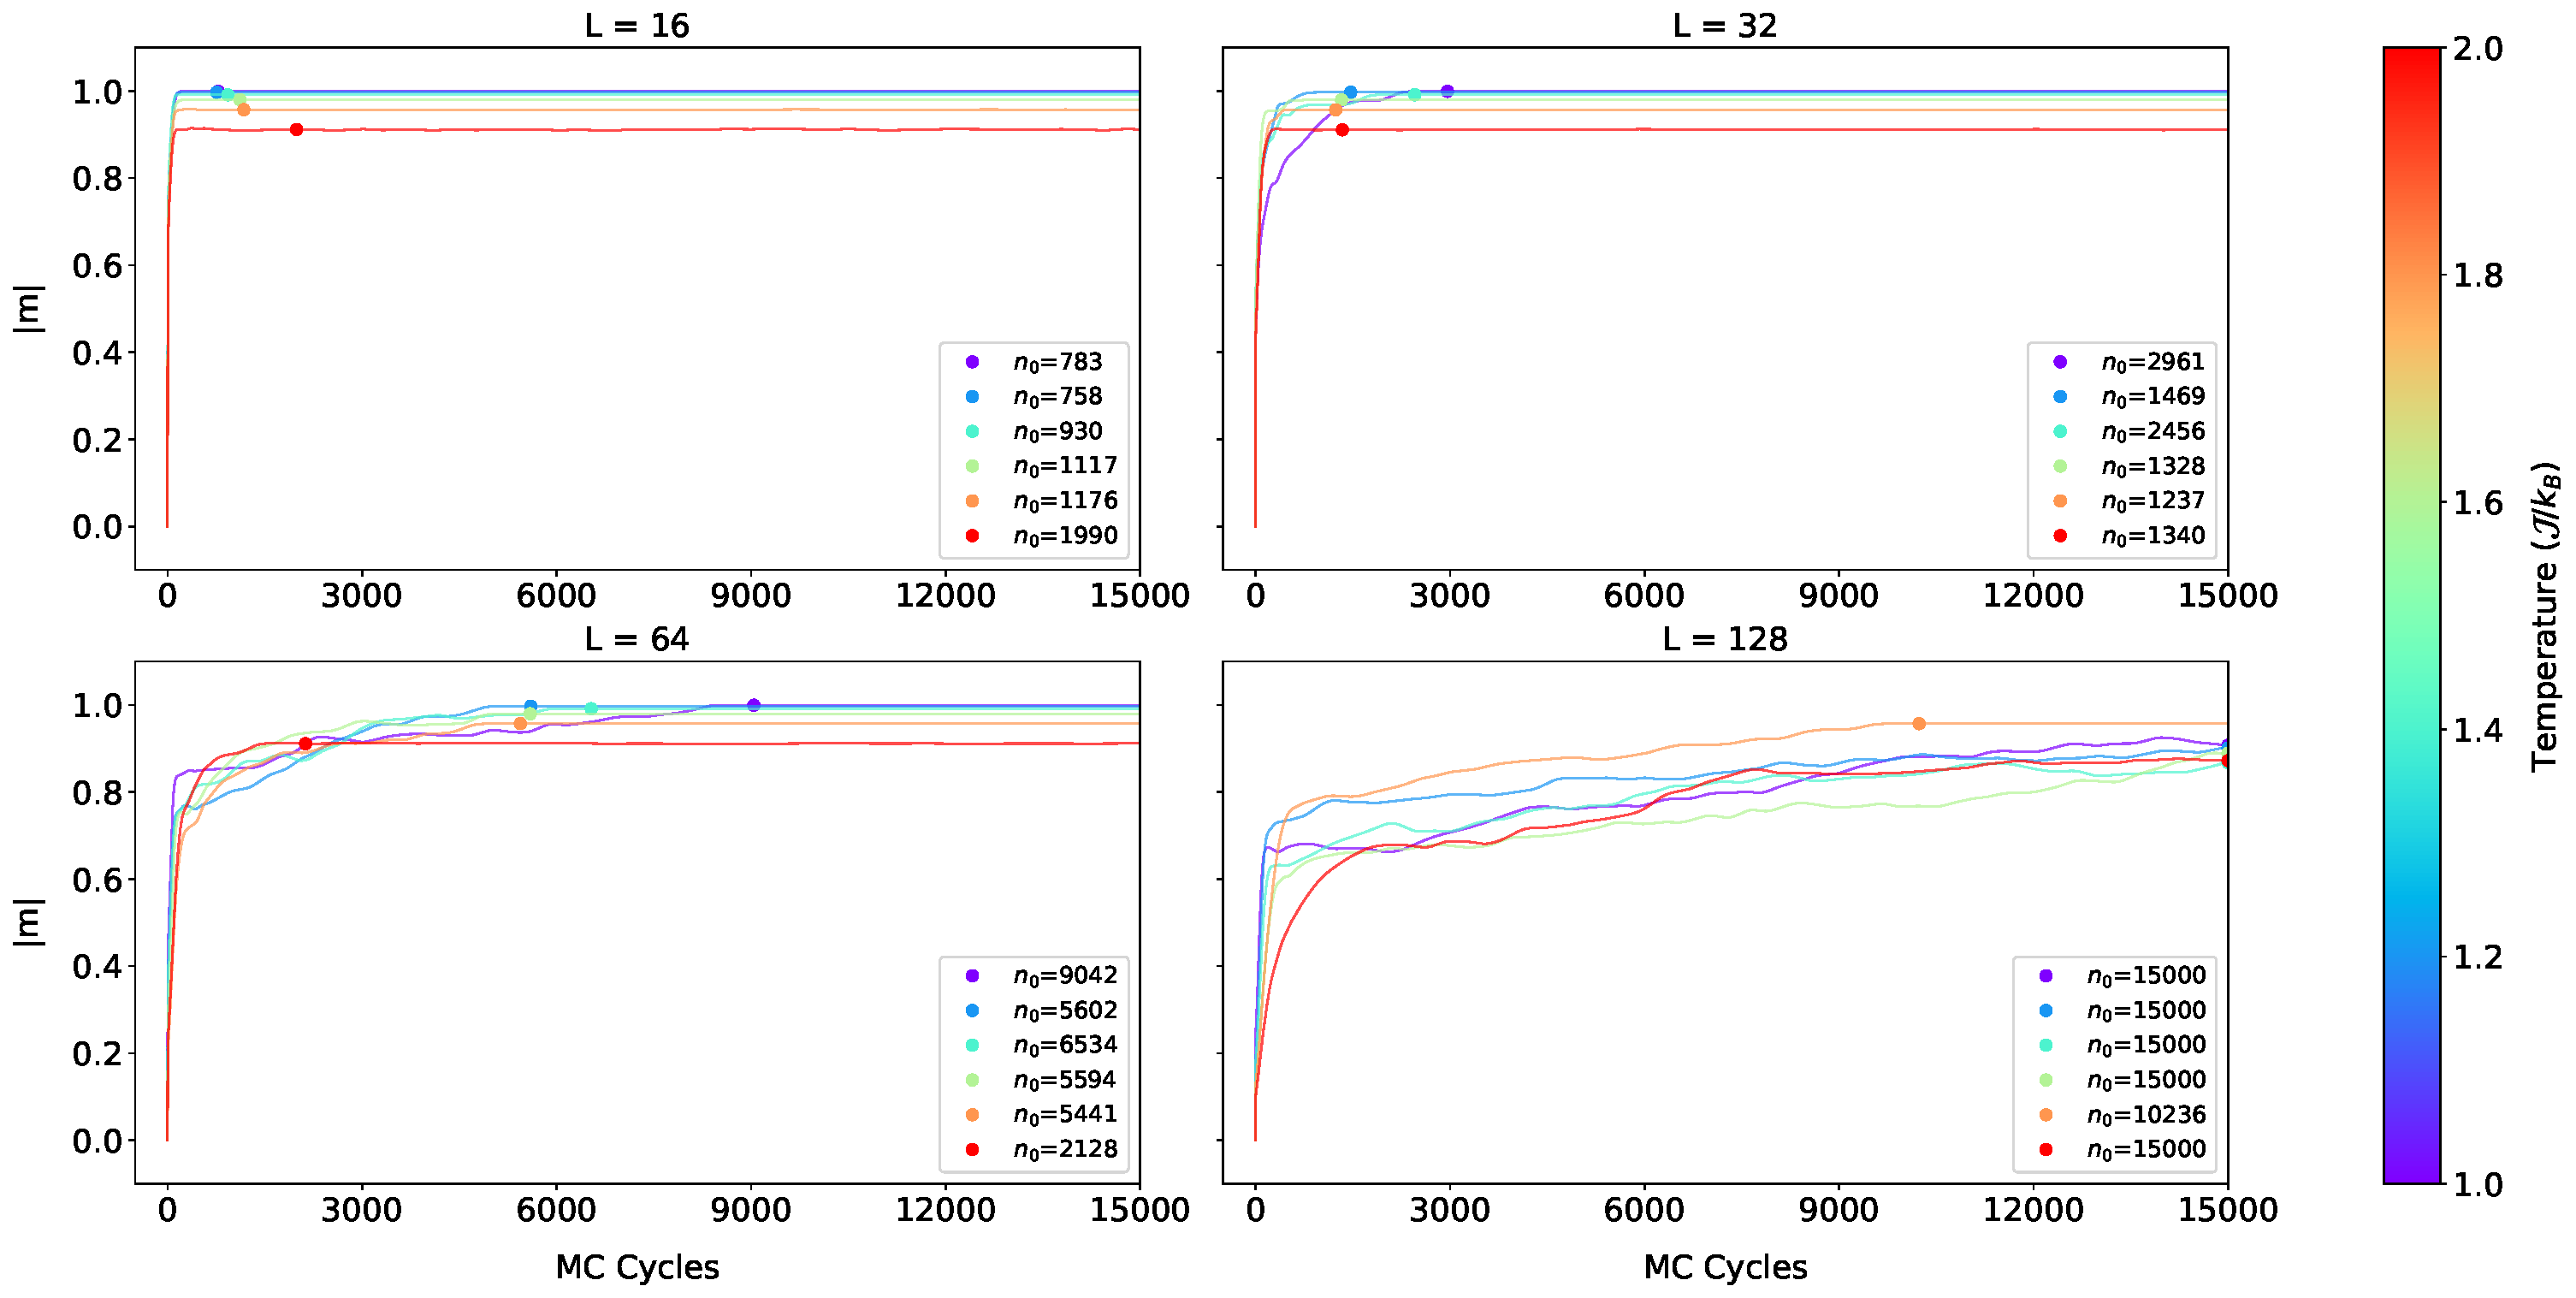
\includegraphics[width=\textwidth]{plots/n0_numpified.pdf}
    \caption{Evolution of absolute magnetization for different temperatures in the range $[1.0,2.0] \ J/k_B$ in increments of $0.2 \ J/k_B$ and spin grid dimension $L = \{2^4,2^5,2^6,2^7\}$ (randomized initial conditions). The data are averaged over 35 simulations and the noise has been filtered out. The equilibration time $n_0$ is defined as the first cycle for which the absolute difference between absolute magnetization values separated by 15 MC cycles remains below a tolerance of $7\times 10^{-5}$ after 750 consecutive intervals.}
    \label{n0_nump}
\end{figure}

\begin{multicols}{2}


\subsection{Observables}

We study the physical observables of (absolute) magnetization, energy per spin, susceptibility per spin, and finally specific heat per spin in different scenarios to assess their behavior and make meaningful connections to the corresponding theory. All the simulations were produced utilizing the numpified version of the Metropolis Algorithm due to reduced computational time.

\subsubsection{Physical Observables vs Temperature}

Firstly, we investigate the behavior of the physical observables as functions of the ratio between temperature and critical temperature $T/T_c$ for different spin grid dimensions and for both $J = \pm 1$. The chosen temperature range corresponds to the vicinity around the critical temperature, where interesting physics happen. The magnetic field is set zero so that we can directly compare the results with the expected behavior described in the theory section, which is derived for $H=0$.\\

Additionally, we expect the results to gradually approach the expected behavior as the dimension of the spin grid grows larger, based on the fact that the theory holds true in the thermodynamic limit $N \to \infty$. In particular, the system cannot support critical fluctuations on length scales larger than $L$, which effectively truncates long-range correlations. As a result, sharp features associated with phase transitions in the thermodynamic limit are increasingly smoothed out as $N \to 0$. We acknowledge this, and expect this behavior to manifest in the results, which are depicted in Fig. (\ref{results1}) for $J=1$.\\

According to the Hamiltonian (Eq. \eqref{hamiltonian}), in the case of positive $J$ the system favors aligned spin configurations (ferromagnetism). Having that in mind, we comment on the results for the different physical observables.\\

\textbf{Absolute Magnetization:} For $T/T_c <1$, the spins are mostly aligned with occasional fluctuations occurring with low probability, and $\braket{|m|} \approx 1$. As $T/T_c \to 1$, the magnetization starts to decrease in a continuous fashion assuming intermediate values ($\braket{|m|}\approx 0.5$), and finally vanishes ($\braket{|m|}\approx 0$) when $T/T_c > 1$, exhibiting a reverse S-shape curve. \\

\begin{figure}[H]
    \centering
    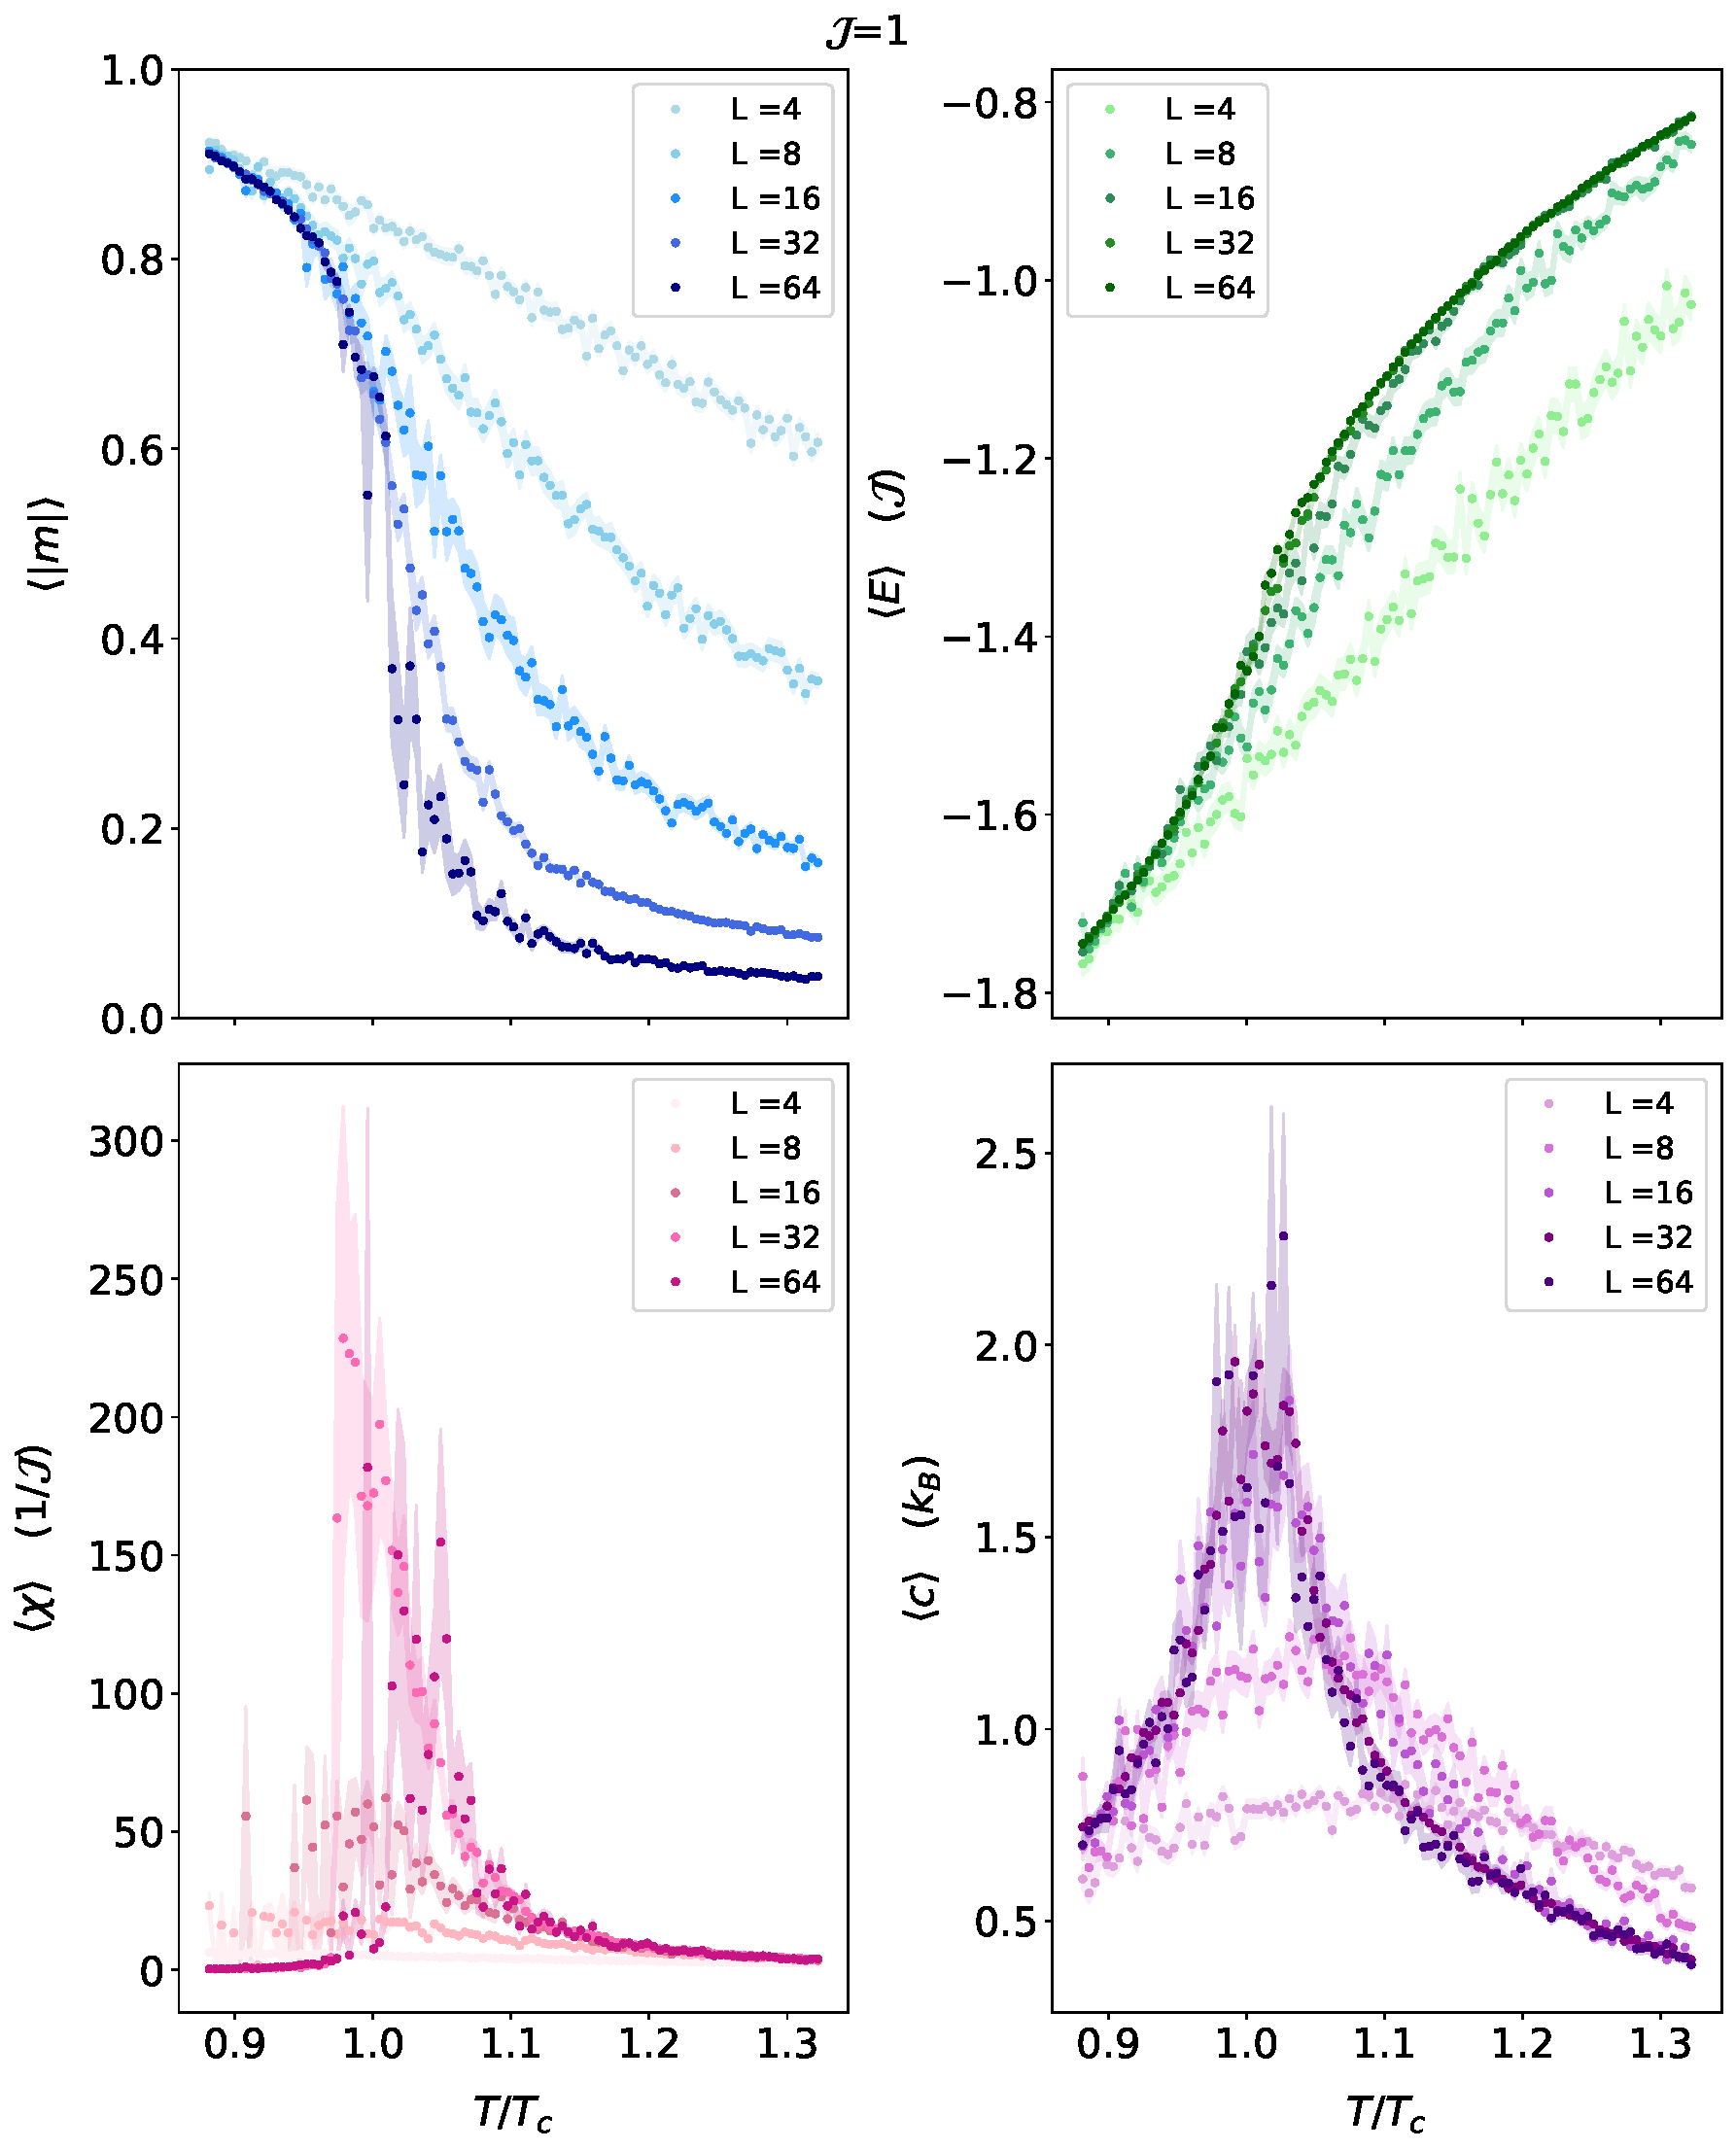
\includegraphics[width=1\columnwidth]{plots/physical_observables_vs_grid.pdf}
    \caption{\textbf{Upper left:} absolute magnetization, \textbf{Upper right:} energy per spin, \textbf{Lower left:} susceptibility per spin, \textbf{Lower right:} specific heat per spin. All the physical observables are plotted as functions of the ratio between temperature and critical temperature $T/T_c$ in the approximate range [0.9,1.3] for $\{L,J,H,n-n_0\} = \{\{2^2,2^3,2^4,2^5,2^6 \},1,0,\{3000,3000,3000,6000,6000\}\}$.}
    \label{results1}
\end{figure}

\textbf{Energy per spin:} For $T/T_c <1$ the energy is close to the theoretical minimum $E_\text{min}/N = -2J = -2$ due to most spins being aligned. As $T/T_c \to 1$, critical fluctuations cause a rapid increase in energy, which eventually slows down towards the maximum value when $T/T_c >1$, because spins are randomly aligned, exhibiting an S-shaped curve.\\ 

\textbf{Susceptibility per spin:} This quantity is a measure of the fluctuations of magnetization, and therefore we can make direct connections between the 2 quantities. For $T/T_c <1$ and $T/T_c>1$, the magnetization is $\braket{m}\approx\pm1$ (or $\braket{|m|}\approx1$) and $\braket{m}\approx0$ respectively. For $T/T_c < 1$, fluctuations occur only occasionally due to decreased probability of spin flips being accepted; for $T/T_c > 1$, spin alignment is random. The preceding discussion manifests as a small and smooth susceptibility in the corresponding regimes. As $T/T_c \to 1$, the emergence of correlated spin domains across the spin grid causes large fluctuations in the magnetization, which appear as a power-law divergence in the susceptibility.\\

\textbf{Specific heat per spin:} This quantity is a measure of the fluctuations of energy, and therefore we can make direct connections between the 2 quantities. For $T/T_c <1$ and $T/T_c>1$, the energy approaches minimization and maximization respectively with minor fluctuations, manifesting as a small and smooth specific heat in these regimes. As $T/T_c \to 1$, the emergence of correlated spin domains across the spin grid causes large energy fluctuations which appear as a logarithmic divergence in the specific heat.\\


The results for $J=-1$ are depicted in Fig. (\ref{results2}). According to the Hamiltonian (Eq. \eqref{hamiltonian}), in the case of negative $J$ the system favors misaligned neighboring spins (anti-ferromagnetism). Having that in mind, we comment on the results for the absolute magnetization and susceptibility per spin, as energy per spin and specific heat per spin are not expected to change with respect to the previous case.\\

\begin{figure}[H]
    \centering
    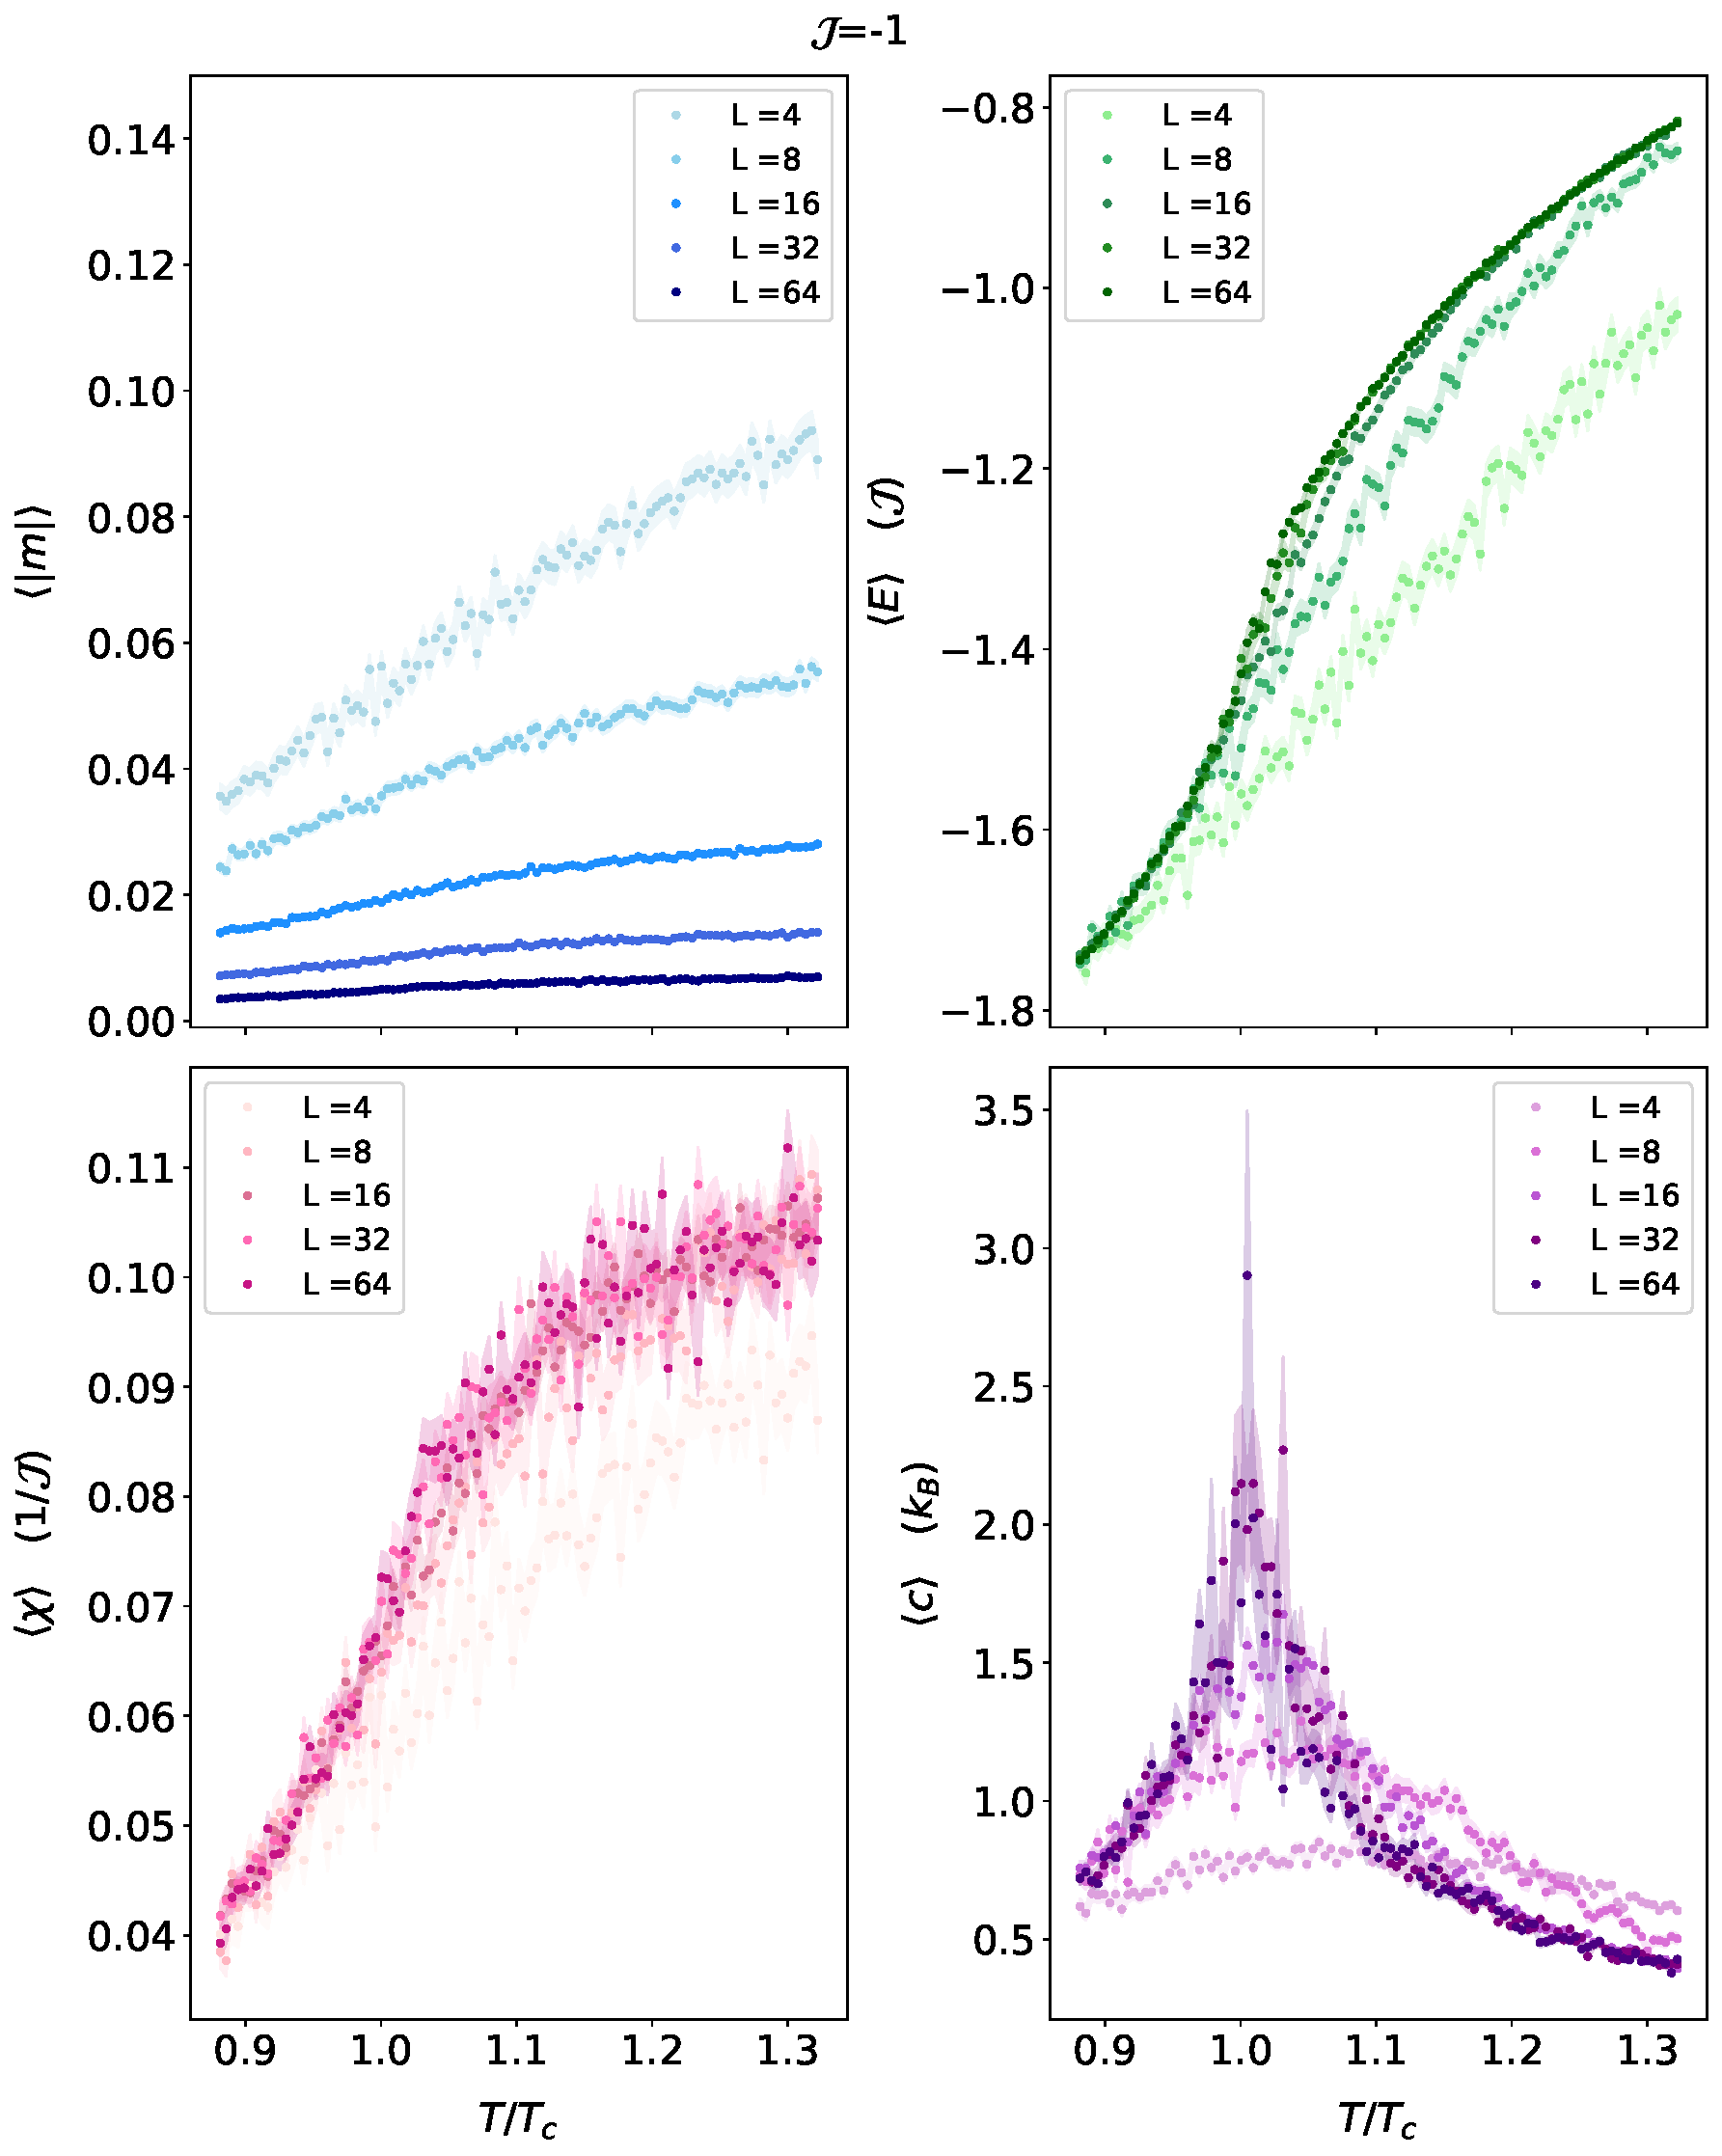
\includegraphics[width=1\columnwidth]{plots/physical_observables_vs_grid_neg_J.pdf}
    \caption{\textbf{Upper left:} absolute magnetization, \textbf{Upper right:} energy per spin, \textbf{Lower left:} susceptibility per spin, \textbf{Lower right:} specific heat per spin. All the physical observables are plotted as functions of the ratio between temperature and critical temperature $T/T_c$ in the approximate range [0.9,1.3] for $\{L,J,H,n-n_0\} = \{\{2^2,2^3,2^4,2^5,2^6 \},-1,0,\{3000,3000,3000,6000,6000\}\}$.}
    \label{results2}
\end{figure}

\textbf{Absolute Magnetization:} Neighboring spins energetically favor anti-alignment, leading to the formation of a checkerboard-like pattern for $T/T_c<1$. Since the up and down spins are approximately equal in this regime, the absolute magnetization approximately vanishes ($\braket{|m|}\approx0$). As $T/T_c \to 1$, critical fluctuations gradually destroy the anti-ferromagnetic alignment, although the absolute magnetization remains small throughout the transition. For $T/T_c > 1$, the spin configuration becomes randomly aligned and $\braket{|m|}\approx0$ continues to hold.\\

\textbf{Susceptibility per spin:} This quantity still reflects fluctuations of the magnetization despite the anti-ferromagnetic behavior. For $T/T_c < 1$, the checkerboard pattern suppresses fluctuations in the magnetization, resulting in a small and smooth susceptibility. As $T/T_c \to 1$, critical fluctuations lead to a gradual increase in the susceptibility. For $T/T_c > 1$, the spins become progressively random, causing the susceptibility to approach a larger but still finite value. However, unlike the ferromagnetic case, this quantity does not fully capture the critical behavior of the system, which is more accurately described by the susceptibility associated with the staggered magnetization, defined as

\begin{align}
    \braket{|m|} = \frac{1}{N} \braket{\big|\sum_\mathbf{x=(i,j)} (-1)^{i+j}s_\mathbf{x}\big|} \in [0,1]
\end{align}
%
and is expected to behave as the regular absolute magnetization in the ferromagnetic case.\\

All of our results are consistent with the theoretical predictions \cite{computational_book}. The increased statistical errors observed near $T/T_c = 1$ arise from critical slowing down and enhanced fluctuations, which lead to longer autocorrelation times and a reduced number of effectively independent MC samples. Additionally, the gradual improvement of the results as spin grid dimension grows larger is consistent with our predictions.

\subsection{Magnetization vs Magnetic Field}
\label{sec_magnetic}

We study the behavior of absolute and proper magnetization as a function of the magnetic field $H$ for different temperatures and $J=1$. The chosen temperature spans the range [0.4,1.3] $T_c$ to investigate the interesting region around the critical temperature. The results are presented in Fig. (\ref{magnetic}).\\

In the upper graph, we observe that the magnetization exhibits an antisymmetric sigmoidal dependence on the magnetic field around $H=0$. For a negative magnetic field the average magnetization is also negative, while for a positive magnetic field it becomes positive, indicating that the external field determines the preferred direction of spin alignment. In the absence of a magnetic field, we recover the behavior discussed previously; zero average magnetization for $T/T_c > 1$ and strong spin ordering for $T/T_c < 1$. A general trend observed across all temperatures is that increasing (decreasing) the magnetic field increases (decreases) the average magnetization, eventually leading to full spin alignment with $\langle m\rangle=1 (-1)$. Furthermore, at higher temperatures, the change in magnetization is more gradual and thus a stronger magnetic field is required to achieve spin ordering, as thermal fluctuations counteract alignment.\\

In the lower graph, we observe that the absolute magnetization exhibits a symmetric dependence on the magnetic field around $H=0$.  For larger magnitudes of the magnetic field, the spins become increasingly aligned, although the increase is more gradual at higher temperatures due to stronger thermal fluctuations. In contrast to the average magnetization, the absolute magnetization at $H=0$ never becomes exactly zero for $T/T_c > 1$, since configurations with opposite magnetization contribute equally to $\langle |m| \rangle$ rather than canceling each other. Nevertheless, $\langle |m| \rangle$ approaches zero as the temperature increases and the system becomes progressively more disordered.

\begin{figure}[H]
    \centering
    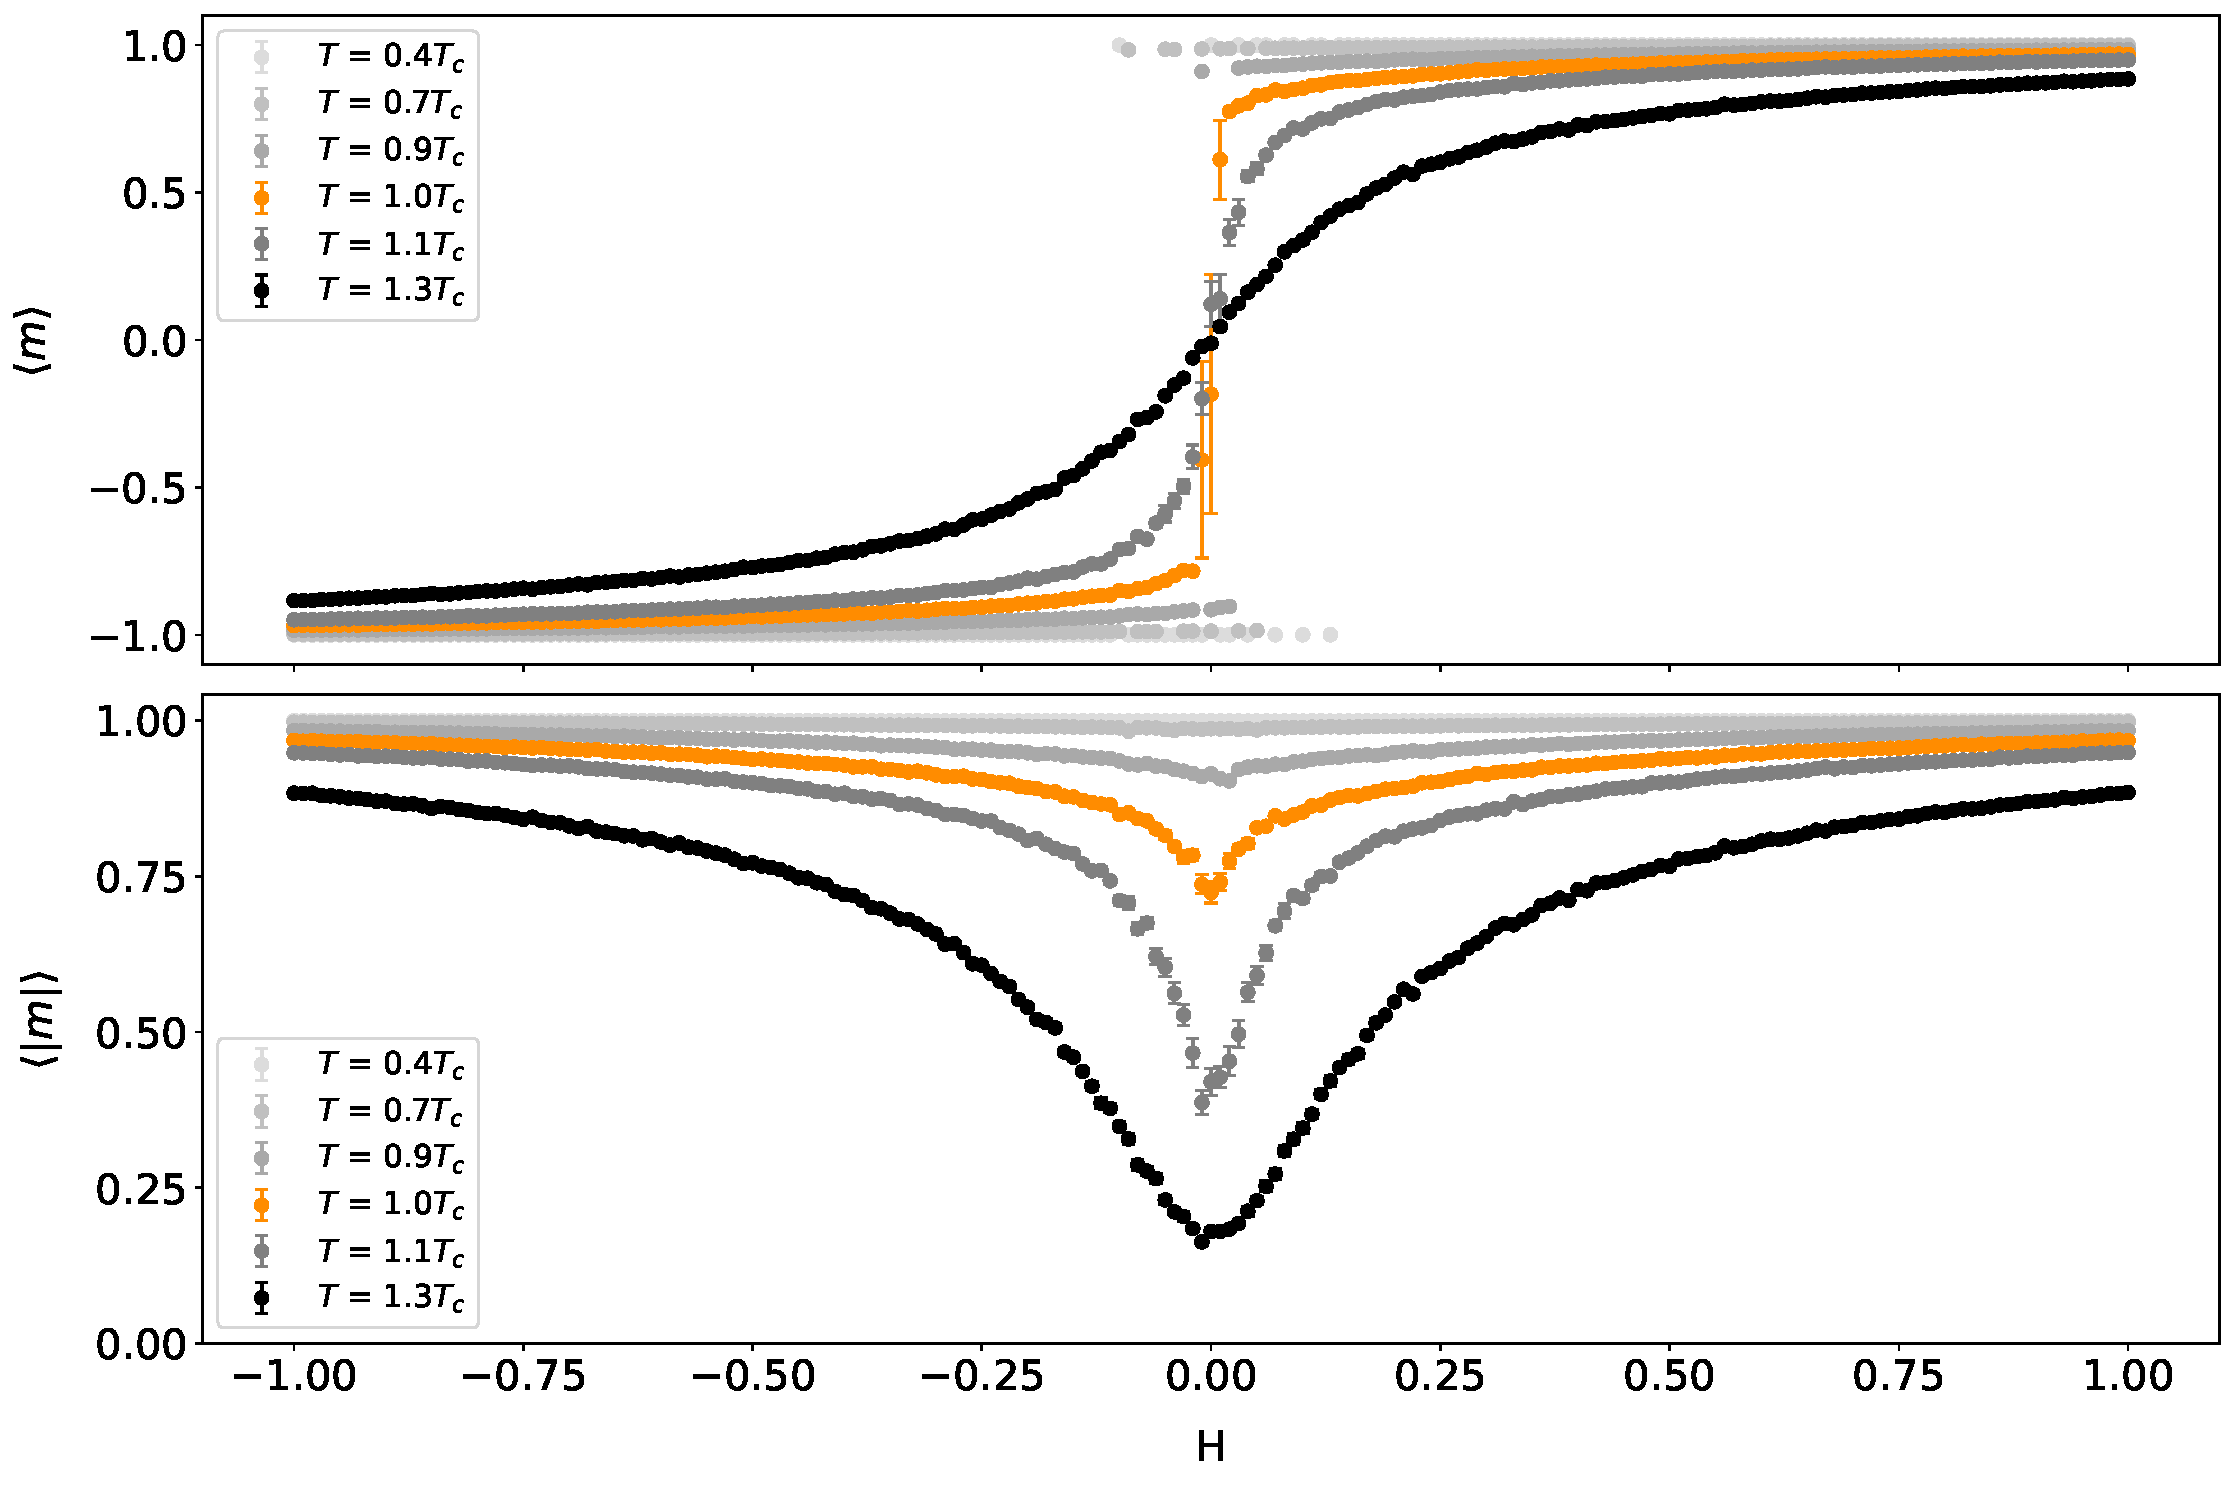
\includegraphics[width=1\columnwidth]{plots/magnetic_field_investigation.pdf}
    \caption{\textbf{Up:} magnetization, \textbf{Down:} absolute magnetization. Both quantities are plotted as functions of the magnetic field $H$ for $\{L,J,n-n_0\}=\{2^4,1,3000\}$}
    \label{magnetic}
\end{figure}

\subsection{Simulation Performance}
\label{sec_performance}

The purpose of implementing the numpified version of the Metropolis Algorithm was to reduce the computational time of the simulation, allowing for the exploration of larger spin grids for more MC cycles in comparison to the standard algorithm. In this section, we quantify the efficiency benefits gained from this implementation.\\

The quantity of interest in our investigation is the computational time $CT$. For both the standard and numpified algorithms, we expect $CT$ to scale with MC cycles $n$ and the spin grid dimension $L$ as

\begin{align*}
    CT \sim \mathcal{O}(nL^2)
\end{align*}

This scaling follows from the structure of the algorithm: for all MC cycles $n$, the algorithm proposes updates over all $N=L^2$ spin sites. Consequently, the computational time can be expressed more formally as

\begin{align}
    CT(n,L) = \alpha L^2\cdot n + \beta,
    \label{comptime}
\end{align}

where $\beta$ is a constant offset associated with fixed overhead
processes such as memory allocation and initialization, and is expected to be negligible for sufficiently large systems and long simulations. Since both implementations exhibit the same functional dependence on $n$ and $L$, the primary factor determining their relative efficiency is the coefficient $\alpha$. To estimate this coefficient, we perform the following procedure for both algorithms:\\

\begin{itemize}
\item[\textbf{(A)}]  We measure the computational time $CT$ as a function of MC cycles $n$ for different fixed values of $L$.

\item[\textbf{(B)}] We fit the measured data with functions $CT_L(n) = (\alpha L^2)\cdot n + \beta$.

\item[\textbf{(C)}] From the fit, we extract the slopes $\left(\frac{\Delta CT}{\Delta n}\right)_L = \alpha L^2$.

\item[\textbf{(D)}]  We plot the slopes as a function of $L$, and fit a quadratic function $\frac{\Delta CT}{\Delta n}(L) = \alpha L^2$.

\item[\textbf{(E)}] From the previous fit, we extract the quadratic coefficient $\alpha$.
\end{itemize}

This coefficient provides insight into how the computational
time of both implementations
scales with the spin grid dimension and the number of MC cycles.
A comparison between the extracted coefficients reveals
the efficiency gain achieved by the numpified version.
The procedure described above is illustrated in Fig. (\ref{performance}), while the resulting coefficients and corresponding speedup are summarized in Tab. (\ref{speedup}).

\begin{table}[H]
    \centering
    \begin{tabular}{|c|c|c|}
    \hline
        $\alpha_\textbf{std}$ (ns) & $\alpha_\textbf{np}$ (ns) & speedup $\alpha_\textbf{std}/\alpha_\textbf{np}$ \\
        \hline
        \hline
         6878 & 28 & $\approx$ 246 \\ 
         \hline
    \end{tabular}
    \caption{The quadratic coefficient of Eq. \eqref{comptime} for the standard and numpified Metropolis Algorithms, and their ratio, which corresponds to the speedup gained from the numpified implementation.}
    \label{speedup}
\end{table}

\end{multicols}

\begin{figure}[h]
    \centering
    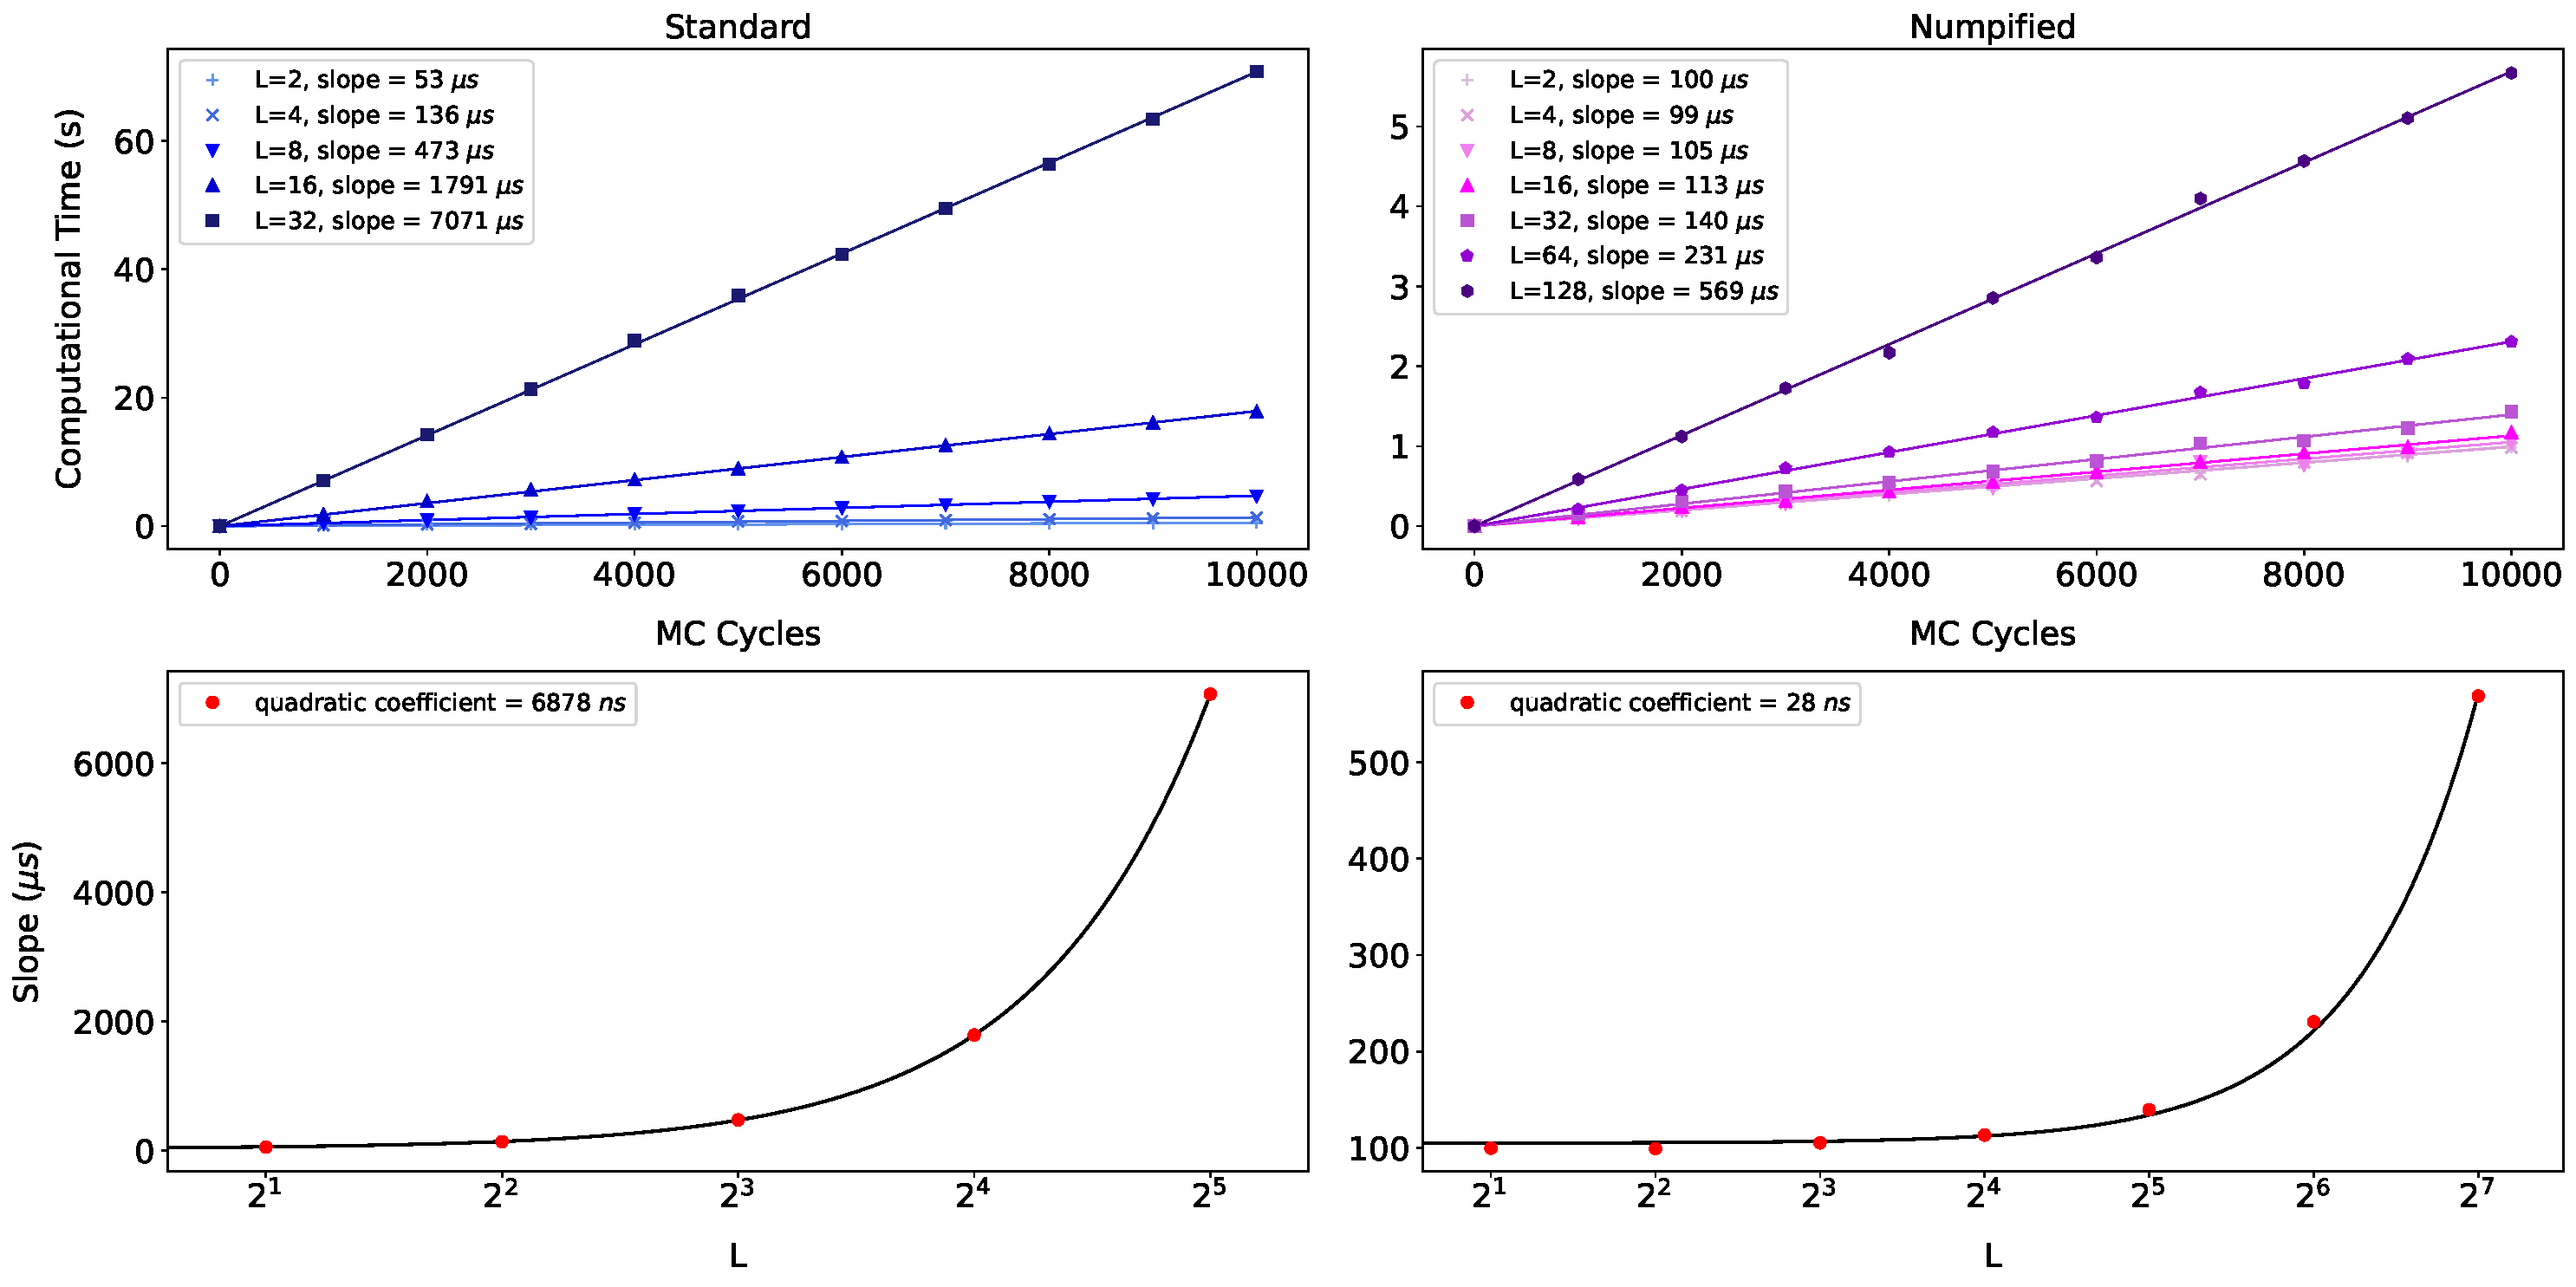
\includegraphics[width=\textwidth]{plots/simulation_performance.pdf}
    \caption{\textbf{Upper left:} Computational time $CT$ as a function of MC cycles $n$ for $L = \{2^1, 2^2,2^3,2^4,2^5\}$ for the \textbf{standard} metropolis algorithm with a linear fit. \textbf{Lower left:} The slope of the fit as a function of $L$. The data were fit with a quadratic function with coefficient $\alpha_\textbf{std} = 6878$ns. \textbf{Upper right:} Computational time $CT$ as a function of MC cycles $n$ for $L = \{2^1, 2^2,2^3,2^4,2^5,2^6,2^7\}$ for the \textbf{numpified} metropolis algorithm with a linear fit. \textbf{Lower right:} The slope of the fit as a function of $L$. The data were fit with a quadratic function with coefficient $\alpha_\textbf{np} = 28$ns.}
    
    \label{performance}
\end{figure}

\begin{multicols}{2}

The results indicate that the numpified Metropolis Algorithm yields a $\times 246$ speedup in computational time. This improvement was crucial for enabling simulations of larger spin lattices, and for measuring observables with higher resolution compared to the standard implementation. The importance of larger systems lies in their ability to more closely approximate the thermodynamic limit $N \to \infty$, for which many analytical results become exact; hence, our numerical results are expected to better reflect the theoretical predictions.


\section{Conclusions}

In summary, we presented a Monte Carlo simulation of the 2D Ising Model with the Metropolis Algorithm, highlighting the relevant methods and theory underlying the setup, initializations, and time-evolution. We extensively discussed the physics and expected behavior of the relevant observables, namely magnetization, energy, susceptibility and specific heat. The numerical results are consistent with the analytical solution of the model, supporting the validity of our implementation. Additionally, we made a brief statement on the estimation of statistical errors, and performed necessary validation checks to ensure that the simulation works reliably. Moreover, we presented insightful results on how the computational time scales with the dimension of the spin lattice and the number of Monte Carlo cycles. Finally, we explored the performance gains from the implementation of the numpified Metropolis Algorithm, and justified how they can help us approach the thermodynamic limit more effectively, revealing more accurate physics.

% ======================
\bibliographystyle{unsrt}
\bibliography{references}
% ======================
\end{multicols}



\end{document}